\documentclass[10pt,twocolumn,letterpaper]{article}

\usepackage{cvpr}
\usepackage{times}
\usepackage{epsfig}
\usepackage{graphicx}
\usepackage{amsmath}
\usepackage{amssymb}
\usepackage[normalem]{ulem}

\usepackage[utf8]{inputenc}
\usepackage{listings}
\usepackage{float}
\usepackage{graphics}
\usepackage{graphicx} 
\usepackage{caption} 
\usepackage{subcaption} 
\usepackage{verbatim}
\usepackage{cite}

% Include other packages here, before hyperref.

% If you comment hyperref and then uncomment it, you should delete
% egpaper.aux before re-running latex.  (Or just hit 'q' on the first latex
% run, let it finish, and you should be clear).
\usepackage[pagebackref=true,breaklinks=true,letterpaper=true,colorlinks,bookmarks=false]{hyperref}

\cvprfinalcopy % *** Uncomment this line for the final submission

\def\cvprPaperID{3265} % *** Enter the CVPR Paper ID here
\def\httilde{\mbox{\tt\raisebox{-.5ex}{\symbol{126}}}}

\newcommand{\kris}[1]{{\color{red} KS: #1}}
\newcommand{\tompson}[1]{{\color{green} JT: #1}}
\newcommand{\herscher}[1]{{\color{blue} SH: #1}}
\newcommand{\edit}[1]{{\color{red} E: #1}}
\newcommand{\cut}[2]{{\color{gray} #1}}

% Pages are numbered in submission mode, and unnumbered in camera-ready
\ifcvprfinal\pagestyle{empty}\fi
\begin{document}
%%%%%%%%% TITLE
%\title{Experiments in Deferred Shading for Training Image Classifiers \tompson{I really don't like the title. Lets chat in person.}}
\title{Beyond Photo Realism For Domain Adapted Synthetic Data}

\author{Kristofer Schlachter\\
NYU\\
{\tt\small schlacht@cims.nyu.edu}
% For a paper whose authors are all at the same institution,
% omit the following lines up until the closing ``}''.
% Additional authors and addresses can be added with ``\and'',
% just like the second author.
% To save space, use either the email address or home page, not both
\and
Connor DeFanti\\
NYU\\
{\tt\small defanti@cims.nyu.edu}
\and
Sebastian Herscher\\
NYU\\
{\tt\small herscher@nyu.edu}
\and
Ken Perlin\\
NYU\\
{\tt\small perlin@nyu.edu}/
\and
Jonathan Tompson\\
Google Brain\\
{\tt\small tompson@google.com}
}

\maketitle
%\thispagestyle{empty}
\maketitle

%%%%%%%%%%%%%%%%%%%%%%%%%%%%%%%%%%%%%%%%%%%%%%%%%%%%%%%%%%%%%%%%%%%%%%%%%%%%%%%%%%%%%%%%%%%%%%%%%%%%%%%%%%%%
%%%%%%%%%%%%%%%%%%%%%%%%%%%%%%%%%%%%%%%%%%%%%%%%%%%%%%%%%%%%%%%%%%%%%%%%%%%%%%%%%%%%%%%%%%%%%%%%%%%%%%%%%%%%
\section{Abstract}
%%%%%%%%%%%%%%%%%%%%%%%%%%%%%%%%%%%%%%%%%%%%%%%%%%%%%%%%%%%%%%%%%%%%%%%%%%%%%%%%%%%%%%%%%%%%%%%%%%%%%%%%%%%%
%%%%%%%%%%%%%%%%%%%%%%%%%%%%%%%%%%%%%%%%%%%%%%%%%%%%%%%%%%%%%%%%%%%%%%%%%%%%%%%%%%%%%%%%%%%%%%%%%%%%%%%%%%%%

As synthetic imagery is used more frequently in training deep models, it is important to understand how different synthesis techniques impact the performance of such models. In this work, we perform a thorough evaluation of the effectiveness of several different synthesis techniques and their impact on the complexity of classifier domain adaptation to the ``real" underlying data distribution that they seek to replicate. In addition, we propose a novel learned synthesis technique to better train classifier models than state-of-the-art offline graphical methods, while using significantly less computational resources.  We accomplish this by learning a generative model to perform shading of synthetic geometry conditioned on a ``g-buffer'' representation of the scene to render, as well as a low sample Monte Carlo rendered image. Our major contributions are (i) a dataset that allows comparison of real and synthetic versions of the same scene, (ii) an augmented data representation that boosts the stability of learning and improves the datasets accuracy, (iii) three different partially differentiable rendering techniques where lighting, denoising and shading are learned, and (iv) we improve a state of the art generative adversarial network (GAN) approach by using an ensemble of trained models to generate datasets that approach the performance of training on real data and surpass the performance of the full global illumination rendering.
%%%%%%%%%%%%%%%%%%%%%%%%%%%%%%%%%%%%%%%%%%%%%%%%%%%%%%%%%%%%%%%%%%%%%%%%%%%%%%%%%%%%%%%%%%%%%%%%%%%%%%%%%%%%
%%%%%%%%%%%%%%%%%%%%%%%%%%%%%%%%%%%%%%%%%%%%%%%%%%%%%%%%%%%%%%%%%%%%%%%%%%%%%%%%%%%%%%%%%%%%%%%%%%%%%%%%%%%%
\section{Introduction}
%%%%%%%%%%%%%%%%%%%%%%%%%%%%%%%%%%%%%%%%%%%%%%%%%%%%%%%%%%%%%%%%%%%%%%%%%%%%%%%%%%%%%%%%%%%%%%%%%%%%%%%%%%%%
%%%%%%%%%%%%%%%%%%%%%%%%%%%%%%%%%%%%%%%%%%%%%%%%%%%%%%%%%%%%%%%%%%%%%%%%%%%%%%%%%%%%%%%%%%%%%%%%%%%%%%%%%%%%

Applying deep learning to supervised computer vision tasks commonly requires large labeled datasets \cite{imagenet, coco}, which can be time consuming, expensive or impractical to collect. As a result, increasingly more synthetic data has been used to overcome these scalability limitations \cite{DBLP:journals/corr/RichterVRK16, DBLP:journals/corr/ShafaeiLS16, DBLP:journals/corr/ZhangSYSLJF16, DBLP:journals/corr/SixtWL17}. However, using synthetic data can introduce problems that arise from the differences in the distributions of the real and synthesized data \cite{2014arXiv1409.7495G}. Usually the best way to reduce the differences is to use the most realistic simulation method available for synthesizing images, in this case a Global Illumination (GI) based renderer such as Mitsuba\cite{Mitsuba}.  Unfortunately, the computational cost of most GI renderers can be prohibitive.  Recently, there has been research into boosting the effectiveness of existing synthetic data\cite{DBLP:journals/corr/ShrivastavaPTSW16}.  However, these new techniques were not benchmarked against real RGB data or against other rendering techniques.

This work explores the effectiveness of various rendering methods, which range from very low to very high computational cost. We compare multiple synthetic rendering methods with the performance obtained using "real" data distribution as an optimal baseline. This is made possible since we annotate an existing image classification dataset (NORB \cite{LeCun:2004:LMG:1896300.1896315}) with pixel aligned geometry labels obtained using a high-quality photometric scanner. We represent the geometry and material information of the RGB scene using a "Geometry Buffer" or "g-buffer", which gives us a standard set of 3D scenes where geometric transformations are frozen in place. By using a g-buffer, we isolate the physical process of shading a surface from the geometric process of geometry pose and projection.  The shading process is also isolates from camera parameters including location, orientation and field of view. This allows us to directly compare different rendering methods and enables us to isolate any performance difference due to shading alone.

Capitalizing on this standard 3D scene representation we setup a number of experiments to compare rendering methods of increasing sophistication and computational cost.  We then measure the benefit of adding certain rendering techniques and see if the computational cost can be justified.  These experiments measure the relative importance of image rendering features. We use a full GI rendering via Mitsuba as the method whose performance we sought to match or surpass.
We are able to do this by using non-standard rendering techniques that involve using convolutional neural nets to learn shading functions.  This is a form of differentiable rendering where the shading is differentiable. Effectively, we use learned shading to denoise low sample count GI rendering and compared it to high sample count images.  We also explore the use of Generative Adversarial Networks to learn shading functions that could render images in unique ways that beat the performance of the most accurate GI output.
%TODO: MENTION GAN ENSEMBLE
\subsection{Contributions}
\begin{enumerate}
\item We provide a dataset that allows the direct comparison of training on real data versus synthetic by including 3D scans of the objects that are in the photographic dataset.
\item We introduce a novel method of using an ensemble of GAN trained generative models to create an augmented dataset.
\item We contribute a thorough comparison of the performance of all the rendering methods with real data.
\end{enumerate}
%%%%%%%%%%%%%%%%%%%%%%%%%%%%%%%%%%%%%%%%%%%%%%%%%%%%%%%%%%%%%%%%%%%%%%%%%%%%%%%%%%%%%%%%%%%%%%%%%%%%%%%%%%%%
%%%%%%%%%%%%%%%%%%%%%%%%%%%%%%%%%%%%%%%%%%%%%%%%%%%%%%%%%%%%%%%%%%%%%%%%%%%%%%%%%%%%%%%%%%%%%%%%%%%%%%%%%%%%
\section{Related Work}
%%%%%%%%%%%%%%%%%%%%%%%%%%%%%%%%%%%%%%%%%%%%%%%%%%%%%%%%%%%%%%%%%%%%%%%%%%%%%%%%%%%%%%%%%%%%%%%%%%%%%%%%%%%%
%%%%%%%%%%%%%%%%%%%%%%%%%%%%%%%%%%%%%%%%%%%%%%%%%%%%%%%%%%%%%%%%%%%%%%%%%%%%%%%%%%%%%%%%%%%%%%%%%%%%%%%%%%%%

Previous papers have used g-buffers to condition a learned generative model for shading. Nalbach et al. \cite{DBLP:journals/corr/NalbachAMSR16} uses a similar model architecture as the denoiser we employ as well as using a g-buffer as input.  The authors use it to learn to approximate screen space shading techniques with a data-driven approach, to see if data driven methods can replicate the standard shading methods used in games. They differ in their approach in that they are optimizing for images looking real to humans and not optimizing the images' utility for training classifiers.
%Loss Functions for Neural Networks for Image Processing 
%Zhao et al. \cite{DBLP:journals/corr/ZhaoGFK15} discusses the motivation of using Structured Similarity (SSIM) as a loss function for image generators. \tompson{Remove this sentence and just add the \\cite to SSIM above.}

%In SimGAN they use data and 4x data.  What they mean is 1/4 of the dataset vs the whole dataset. Which is not the same as creating more novel data from GANs.\\

There have been recent advances in denoising low sample count images calculated by Global Illumination (GI) based renderers.
%Spatiotemporal Variance-Guided Filtering: Real-Time Reconstruction for Path-Traced Global Illumination 
Shied et al. \cite{Schied:2017:SVF:3105762.3105770} denoises low sample count GI images by combining neighboring frames and feeding them into a fixed spatio-temporal filter.  The authors emphasis is on temporal stability, efficient computation and denoising single sample frames in real-time. Their authors do not employ machine learning in their method. 
%Interactive Reconstruction of Monte Carlo Image Sequences using a Recurrent Denoising Autoencoder 
Chaitanya et al. \cite{Chaitanya:2017:IRM:3072959.3073601} along with 
%Kernel-Predicting Convolutional Networks for Denoising Monte Carlo Renderings 
Bako et al. \cite{Bako17} and 
%A Machine Learning Approach for Filtering Monte Carlo Noise
Kalantari et al. \cite{Kalantari:2015:MLA:2809654.2766977} all use machine learning to denoise Monte Carlo (GI) renderings for graphics applications.  Our work uses a modified form of the model presented in \cite{Chaitanya:2017:IRM:3072959.3073601} in order to denoise images used for training classifiers with the goal of synthesizing training data faster. 

Further use of global illumination for training classifiers has been explored.
%Physically-Based Rendering for Indoor Scene Understanding Using Convolutional Neural Networks 
Zhang et al. \cite{DBLP:journals/corr/ZhangSYSLJF16} use a custom created large 3D indoor dataset to conduct experiments relating the performance of different renderers and lighting for various machine learning tasks, such as normal estimation, semantic segmentation, and object boundary detection. Our approach, in contrast, focuses mainly on shading and its effect on training data quality. 


%Model-driven Simulations for Deep Convolutional Neural Networks 
%REMOVING BECAUSE OF SPACE:Veeravasarapu et al. \cite{DBLP:journals/corr/VeeravasarapuRR16} discuss Monte Carlo methods for generating synthetic data, and they examine several different simulated datasets. They tested various different levels of fidelity (measured in samples-per-pixel) and concluded that beyond a certain threshold (40 spp for their specific scenes), increases in rendering fidelity do not increase the data training accuracy. We build upon this result by using learning-based methods to improve the accuracy of visual fidelity for lower sample counts.

% How useful is photo-realistic rendering for visual learning? 
%REMOVING BECAUSE OF SPACE:Movshovitz-Attias et al. \cite{DBLP:journals/corr/Movshovitz-Attias16} demonstrated that synthetic data produced by a high-quality renderer, when added to a dataset of natural images, can produce training accuracies that are competitive with a larger dataset of real data. Their work focused on rendering parameters, such as lighting positions, background, and camera shutter speed. As opposed to these variables, our work focuses on different methods of rendering light interaction and propagation.

%Playing for Data: Ground Truth from Computer Games
%Play and Learn: Using Video Games to Train Computer Vision Model 
Using a video game engine for dataset creation has been explored by Richter et al. \cite{DBLP:journals/corr/RichterVRK16} and  Shafaei et al. \cite{DBLP:journals/corr/ShafaeiLS16}. They explored the use of video game snapshots to show that it could train image segmentation models. We built upon their approach by using learned rendering techniques to improve the synthesis quality and to decrease rendering computational cost.

%Conditional Image Synthesis with Auxiliary Classifier GANs \cite{DBLP:journals/corr/OdenaOS16} uses label data to improve the results of GANs.  They also use SSIM as a way to measure their results which we attempt to do as well.

%Generative Image Modeling using Style and Structure Adversarial Networks 
To learn shading, we used Generative Adversarial Networks (GANs) which were first introduced by Goodfellow et al. \cite{goodfellow}. Since then many works have used them to synthesize images. 

%Wang and Gupta \cite{DBLP:journals/corr/WangG16} used multiple GANs for unsupervised learning on real data, separating structure and style of the image data into two separate GANs and later recombining the results. This method was applied to data retrieval for images and classification performance was not measured.

%RenderGAN: Generating Realistic Labeled Data 
Learning, partially differentiable renderers was proposed by Sixt et al. \cite{DBLP:journals/corr/SixtWL17}. In their paper they train a differentiable 3D renderer, except their model is scene and application specific. The differentiable rendering model architecture we implemented is not restricted to a specific shading model, geometric input or lighting condition.

%Learning from Simulated and Unsupervised Images through Adversarial Training 
A GAN based method that uses unlabeled data to refine realistic rendered images was pioneered by
Shrivastava et al. \cite{DBLP:journals/corr/ShrivastavaPTSW16}. The paper proposes an architecture that takes in rendered images and makes them more realistic by using an adversarial loss to tune a refiner model. We use this paper as a starting point for our GAN experiments; however, we modify many aspects of it to suit our input which is an g-buffer not just an image.

A GAN-based method related to Shrivastava et al. is Bousmalis et al. \cite{Bousmalis2016UnsupervisedPD}. This paper proposes a very similar method, but conditions the input with a noise vector and a depth buffer.  The depth buffer is used to mask out the background so the refiner network can concentrate upon pixels containing the object to be classified.  Our method conditions on more data including normals and albedo and doesn't mask out parts of the image which allows for shadowing to be modeled. We also improve upon these two papers by using an ensemble of trained GAN generative models to boost training data performance.

%Unsupervised Domain Adaptation by Backpropagation 
%Domain adaptation without modifying the dataset itself is discussed by Ganin and Lempitsky \cite{2014arXiv1409.7495G} who modify the gradients of a classifier during learning in order to make the learned model domain invariant.  

%Generative Adversarial Nets \cite{2014arXiv1406.2661G}\\
%Learning Methods for Generic Object Recognition with Invariance to Pose and Lighting \cite{LeCun:2004:LMG:1896300.1896315}\\

%%%%%%%%%%%%%%%%%%%%%%%%%%%%%%%%%%%%%%%%%%%%%%%%%%%%%%%%%%%%%%%%%%%%%%%%%%%%%%%%%%%%%%%%%%%%%%%%%%%%%%%%%%%%
\subsection{Rendering Methods and Techniques}
%%%%%%%%%%%%%%%%%%%%%%%%%%%%%%%%%%%%%%%%%%%%%%%%%%%%%%%%%%%%%%%%%%%%%%%%%%%%%%%%%%%%%%%%%%%%%%%%%%%%%%%%%%%%

%%%%%%%%%%%%%%%%%%%%%%%%%%%%%%%%%%%%%%%%%%%%%%%%%%%%%%%%%%%%%%%%%%%%%%%%%%%%%%%%%%%%%%%%%%%%%%%%%%%%%%%%%%%%
\subsubsection{G-Buffer}
%%%%%%%%%%%%%%%%%%%%%%%%%%%%%%%%%%%%%%%%%%%%%%%%%%%%%%%%%%%%%%%%%%%%%%%%%%%%%%%%%%%%%%%%%%%%%%%%%%%%%%%%%%%%

G-Buffers \cite{Saito:1990:CRS:97879.97901} separate the geometric processes such as transformation, projection and depth testing, from physical processes such as shading and texture mapping. This is accomplished by the buffers accumulating the geometry information in the first pass and then lighting each pixel of the output on a second pass (which is linear in both model and lighting complexity).  This is in comparison to a forward renderer which calculates geometry information and performs lighting and shadowing in one pass (with quadratic complexity), followed by and writing the result to the output buffer. This technique of using G-Buffers and screen-space rendering is known as ``deferred shading,'' where expensive lighting and shadowing computation is done after all of the visible geometry is encoded into its buffers.
 As an added benefit for this work, the encoding of our geometry state into G-Buffers allows for simplified testing of different shading techniques on the identical 3D scenes.
In our experiments, our G-Buffer consists of the scene encoded geometry normals, geometry diffuse color (also referred to as albedo), and the linear depth from the camera to the visible geometry.  See figure \ref{fig:GBUFFER_ALBEDO}, for examples. We describe how the datasets are produced in \ref{TrainingData}.

\begin{figure}[h!]
\centering
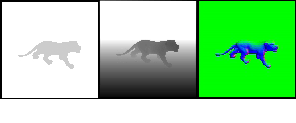
\includegraphics[width=0.8\columnwidth]{./assets/gbuffer-onerow.png}
\caption{G-Buffer. Left is Albedo, middle is Depth, right is world space Normals.}
\label{fig:GBUFFER_ALBEDO} 
\end{figure}

%%%%%%%%%%%%%%%%%%%%%%%%%%%%%%%%%%%%%%%%%%%%%%%%%%%%%%%%%%%%%%%%%%%%%%%%%%%%%%%%%%%%%%%%%%%%%%%%%%%%%%%%%%%%
\subsubsection{Spherical Harmonics}
%%%%%%%%%%%%%%%%%%%%%%%%%%%%%%%%%%%%%%%%%%%%%%%%%%%%%%%%%%%%%%%%%%%%%%%%%%%%%%%%%%%%%%%%%%%%%%%%%%%%%%%%%%%%
\begin{figure}[h!]
\centering
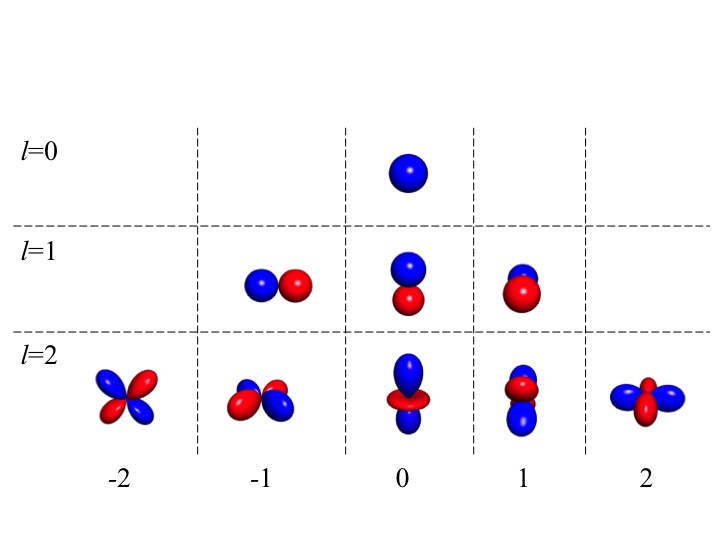
\includegraphics[width=1.0\columnwidth]{./assets/SH_Fig.jpg}
\caption{Visualization of first 3 bands of the spherical harmonics functions. Red are negative values and blue are positive. These are the corresponding 9 functions to the 9 coefficients we learn for lighting.}
\label{fig:SHBands01}
\end{figure}

In our experiments, we use a set of functions called Spherical Harmonics (SH) to learn the lighting of an environment. Spherical Harmonics are a set of continuous and rotationally invariant functions that approximate an arbitrary spherical function, such as the distribution of light reflected off of a surface \cite{Ramamoorthi:2001:ERI:383259.383317}, also known as a bidirectional reflectance distribution function (BRDF). The orthogonal functions are grouped into levels of increasing detail, resolution, or frequency. SH are grouped into levels, where each level is a set of orthogonal functions of finer detail, resolution, or frequency \cite{Shreiner:2013:OPG:2544032}.  To represent the smooth lighting in our experiments, we only need the first three levels which are a constant, linear polynomials, and quadratic polynomials of the surface normal. See Figure \ref{fig:SHBands01} for a visualization of the first three levels.

Using Spherical Harmonics for lighting allows for a 9-float representation of a smooth lighting environment. We use SH to represent complex lighting models in a compressed form, which has the effect of drastically reducing the search space when trying to learn a parameterized lighting model.

An advantage to using Spherical Harmonics for lighting is that you can represent a smooth lighting environment with just 9 floats. This allows us to parameterize a lighting function with far fewer parameters compared to other representations. This has the effect of drastically reducing the search space when trying to learn a parameterized lighting model.

We create trainable module that calculates three levels of SH basis functions. The input to the module consists of the surface normal at every pixel, which is conveniently stored in the G-Buffer. The network outputs a shaded image which can be composited with shadowing and albedo.

%%%%%%%%%%%%%%%%%%%%%%%%%%%%%%%%%%%%%%%%%%%%%%%%%%%%%%%%%%%%%%%%%%%%%%%%%%%%%%%%%%%%%%%%%%%%%%%%%%%%%%%%%%%%
\subsubsection{Ambient Occlusion}
%%%%%%%%%%%%%%%%%%%%%%%%%%%%%%%%%%%%%%%%%%%%%%%%%%%%%%%%%%%%%%%%%%%%%%%%%%%%%%%%%%%%%%%%%%%%%%%%%%%%%%%%%%%%

In an environment with only large area light sources, there exists a simple first order approximation to global illumination called Ambient Occlusion. It is used a form of simplified global illumination because it takes into account only screen-space visible  scene geometry\cite{Miller:1994:EAL:192161.192244}.  Each view-ray from the camera's pixel samples defines a single point on the surface of the scene geometry. The algorithm uses these local screen-space geometry samples to approximate how exposed each surface fragment is incoming ambient light sources by estimating how much of the hemisphere around that point is blocked by nearby surfaces. 
%For lighting conditions that are close to a uniformly bright hemisphere, like an overcast day, then ambient occlusion is a good approximation of global illumination.
%This method fails in scenes and camera positions where light occluding geometry that is not-visible to the camera projection dominate the illumination function \tompson{When else does this fail?}. 

%%%%%%%%%%%%%%%%%%%%%%%%%%%%%%%%%%%%%%%%%%%%%%%%%%%%%%%%%%%%%%%%%%%%%%%%%%%%%%%%%%%%%%%%%%%%%%%%%%%%%%%%%%%%
\subsubsection{Global Illumination}\label{mitsuba_section}
%%%%%%%%%%%%%%%%%%%%%%%%%%%%%%%%%%%%%%%%%%%%%%%%%%%%%%%%%%%%%%%%%%%%%%%%%%%%%%%%%%%%%%%%%%%%%%%%%%%%%%%%%%%%

Global illumination (GI) refers to rendering methods that take into account inter-surface reflection, to significantly improved visual fidelity in comparison to faster approximate methods that only simulate direct lighting (or limited bounce counts).  GI derives its accuracy from its ability to take into account the light that arrives at a surface not just directly from a light source, but from light that has been reflected off of other surfaces as well. Different surface materials have different reflection characteristics that effect how much sampling must be done in order to converge to the right solution. We chose a classification dataset with homogeneous and simple material properties, such that all of the dataset is diffuse and there are few surfaces capable of reflecting light onto the objects in the scene. We made this decision to avoid the typical thousands of iterations necessary to get a noise free image\footnote{Usually for scenes with highly reflective surfaces and small bright light sources}.

%In order to simulate global illumination in our experiments, we used the open source global illumination renderer, Mitsuba.  It generates high quality images that it creates by solving the rendering equation by bouncing many light rays throughout the 3D scene.  The more samples it takes, the closer to the solution and the more realistic the image becomes, but at the cost of high computation; images rendered by Mitsuba often take many orders of magnitude longer than with rasterization methods such as ones included in OpenGL.  

%%%%%%%%%%%%%%%%%%%%%%%%%%%%%%%%%%%%%%%%%%%%%%%%%%%%%%%%%%%%%%%%%%%%%%%%%%%%%%%%%%%%%%%%%%%%%%%%%%%%%%%%%%%%
\section{Training Data Creation}\label{TrainingData}
%%%%%%%%%%%%%%%%%%%%%%%%%%%%%%%%%%%%%%%%%%%%%%%%%%%%%%%%%%%%%%%%%%%%%%%%%%%%%%%%%%%%%%%%%%%%%%%%%%%%%%%%%%%%
Direct comparisons between rendering techniques and real images could not be done without creating a dataset that has approximately 1:1 correspondence between domains.  To this end we identified the NYU Object Recognition Benchmark (NORB) dataset \cite{LeCun:2004:LMG:1896300.1896315} as a good starting point. It is small enough to allow for recreation of each photograph with high accuracy in simulation.  A characteristic that makes NORB even more attractive is that the object location, rotation, camera placement and lighting condition are known for every image. Furthermore, each object was modified so that the BRDF of each object was approximately homogeneous across the dataset.

However, the NORB dataset is comprised of grayscale images, which is less-relevant for modern deep-learning architectures. As such, we composed an additional dataset of synthetic objects from ShapeNet~\cite{DBLP:journals/corr/ChangFGHHLSSSSX15} (choosing a disjoint set of object classes), where the ground-truth RGB image is the result of our most expensive offline rendering method available. This dataset was digital-only and did not have physical models that we could scan like the NORB dataset. So, we used synthetic renders for both training the learning model and testing its accuracy.

While this is not sufficient on its own to make conclusions about our learning model on real image data, we use this additional synthetic dataset to validate our grayscale NORB results on a RGB dataset of similar complexity and composition. %TODO: reread this?

%%%%%%%%%%%%%%%%%%%%%%%%%%%%%%%%%%%%%%%%%%%%%%%%%%%%%%%%%%%%%%%%%%%%%%%%%%%%%%%%%%%%%%%%%%%%%%%%%%%%%%%%%%%%
\subsection{NORB Dataset}\label{NORB-DATASET}
%%%%%%%%%%%%%%%%%%%%%%%%%%%%%%%%%%%%%%%%%%%%%%%%%%%%%%%%%%%%%%%%%%%%%%%%%%%%%%%%%%%%%%%%%%%%%%%%%%%%%%%%%%%%
\begin{figure}[h!]
\centering
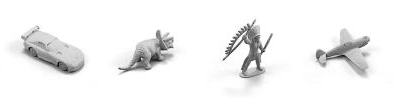
\includegraphics[width=1.0\columnwidth]{./assets/NORBTestSmall.png}
\caption{A sample of the NORB test dataset. Note the dark shadows under some of the models, animals in particular.}
\label{fig:norb-samples}
\end{figure}
%TODO: figure vspace?

The NORB dataset consists of a set of 50 toys split into a 25 object training set and a 25 object test set. For each object, stereo photographs were taken with the object on a turntable in 6 controlled lighting conditions and with 18 camera azimuth angles and 9 elevation angles. This results in a dataset with 48,600 stereo pictures.  We limited our use of the dataset to just the 25 objects in the training set. We also confined our dataset to one lighting condition, reducing the image count in the training dataset to 4,050 images. The toys were painted a uniform color with a matte paint. This was intended to prevent texture from being used in classification.

 All of the properties listed above facilitate a near-perfect recreation of the original scenes through 3D rendering (whereas it would be significantly more complicated to recreate natural outdoor scenes with perfect 1:1 geometry correspondence). We know the pose, location and surface of the objects as well as the location of the camera. We set the material properties based on the paint used for the physical toy models.
 %of the objects to be a uniform color hand-chosen to match the NORB model color and diffusely reflective.
 
We used the HP 3D Structured Light Scanner Pro S3\cite{HPSCANNER} to scan in the objects. The models were then uniformly scaled to fit into a unit cube with the bottom center at the origin. We then rendered a matching g-buffer for every image in the training dataset.  

Mitsuba produced the G-Buffers and shaded images at a resolution of 768x768 for each image.  The images and buffers were then cropped and resized such that the bounding box of the mesh pixels fit into an 80x80 pixel square, with the final image itself being a 96x96 pixel square. This mirrors the procedure done for the source NORB dataset. This creation procedure results in a one-to-one mapping between each image in the synthetic training dataset with the corresponding ``real'' image in the NORB training dataset.
%As briefly mentioned, the NORB dataset does have its shortcomings when compared to recent deep-learning datasets of significantly larger size. The dataset is black and white, low resolution, has very little visual variety and it small in number of samples. While these are drawbacks, the dataset was generated using a controlled capture environment, which helps us eliminate variables such as bad lighting or background noise when evaluating our learning model. Therefore, we can conduct experiments comparing only rendering variables, such as lighting, rendering methods, and more. These conditions are detailed later.
%%%%%%%%%%%%%%%%%%%%%%%%%%%%%%%%%%%%%%%%%%%%%%%%%%%%%%%%%%%%%%%%%%%%%%%%%%%%%%%%%%%%%%%%%%%%%%%%%%%%%%%%%%%%
\subsection{ShapeNet Dataset}
%%%%%%%%%%%%%%%%%%%%%%%%%%%%%%%%%%%%%%%%%%%%%%%%%%%%%%%%%%%%%%%%%%%%%%%%%%%%%%%%%%%%%%%%%%%%%%%%%%%%%%%%%%%%

\begin{figure}[h!]
\centering
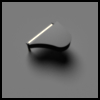
\includegraphics[width=0.24\columnwidth]{./assets/piano.jpg}
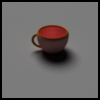
\includegraphics[width=0.24\columnwidth]{./assets/mug.jpg}
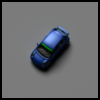
\includegraphics[width=0.24\columnwidth]{./assets/car.jpg}
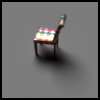
\includegraphics[width=0.24\columnwidth]{./assets/chair.jpg}
\caption{A sample of our ShapeNet train dataset.}
\label{fig:SHAPENET}
\end{figure}

  The ShapeNet dataset consists of tens of thousands of models. For our tasks, we took a subset of ShapeNet, taking 10 different models from 10 categories each. The dataset size was chosen to match similar popular, small datasets CFAR-10 \cite{Krizhevsky09learningmultiple} and MNIST \cite{726791}. The categories we chose were airplanes, boats, cars, chairs, motorcycles, mugs, pianos, planters, tables, and trains. This provided a wide variety of models that could be identified from many different camera angles. 

After each model was changed to fit the above conditions, they were then rendered using the Mitsuba renderer. An infinitely large, matte ground plane was created below the objects, and two large, spherical area lights were created above the object to create shadows. In a specific experiment, detailed later, these lights were replaced by a single directional light to create harder shadows. For each model, we used 162 randomly sampled camera angles. The camera angles were chosen such that the elevation angles were between 30 and 70 degrees, and the azimuth could be any angle (between 0 and 2$\pi$ radians). These bounds and the number of samples were chosen to best match the NORB dataset. The randomization was chosen uniformly, such that if $\zeta_1\in[\cos(70^\circ),\cos(30^\circ)],\zeta_2\in[0,1]$ are uniformly distributed random numbers, then the elevation angle $\theta$ and azimuth angle $\phi$ are $\theta = \cos^{-1}\zeta_1$, $\phi = 2\pi \zeta_2$. This follows the formula given by \cite{Pharr:2010:PBR:1854996}. The images were rendered at 96x96, outputting the G-buffer of each image, including the image albedo, normals, occlusion, distance field, and color image data.

%%%%%%%%%%%%%%%%%%%%%%%%%%%%%%%%%%%%%%%%%%%%%%%%%%%%%%%%%%%%%%%%%%%%%%%%%%%%%%%%%%%%%%%%%%%%%%%%%%%%%%%%%%%%
\section{Experiments}
%%%%%%%%%%%%%%%%%%%%%%%%%%%%%%%%%%%%%%%%%%%%%%%%%%%%%%%%%%%%%%%%%%%%%%%%%%%%%%%%%%%%%%%%%%%%%%%%%%%%%%%%%%%%

In our experiments, we use increasingly complex simulation methods for rendering our images.  We start with just a silhouette as training data and we then incrementally increase the sophistication level of the rendering.  We then add complexity such as shading, shadowing and global illumination. Finally, we use a form of a denoising autoencoder to learn cleanup and refine GI based images.% \footnote{See figure \ref{fig:denoise} and section \ref{denoising} for denoiser details}.

In order to principally measure the impact of these various techniques, we use a single classifier architecture across all experiments; a simplification of the VGG network\cite{DBLP:journals/corr/SimonyanZ14a}. Given the small size of our datasets, we reduce the standard VGG network to 8 learnable layers, including 5 convolutional and 3 fully-connected layers. We then use a cross-entropy loss (i.e. negative log likelihood) to train the 5-class output. See 
Figure~\ref{fig:VGG_DAIGRAM} for an overview of this architecture.

\begin{figure}[h!]
\centering
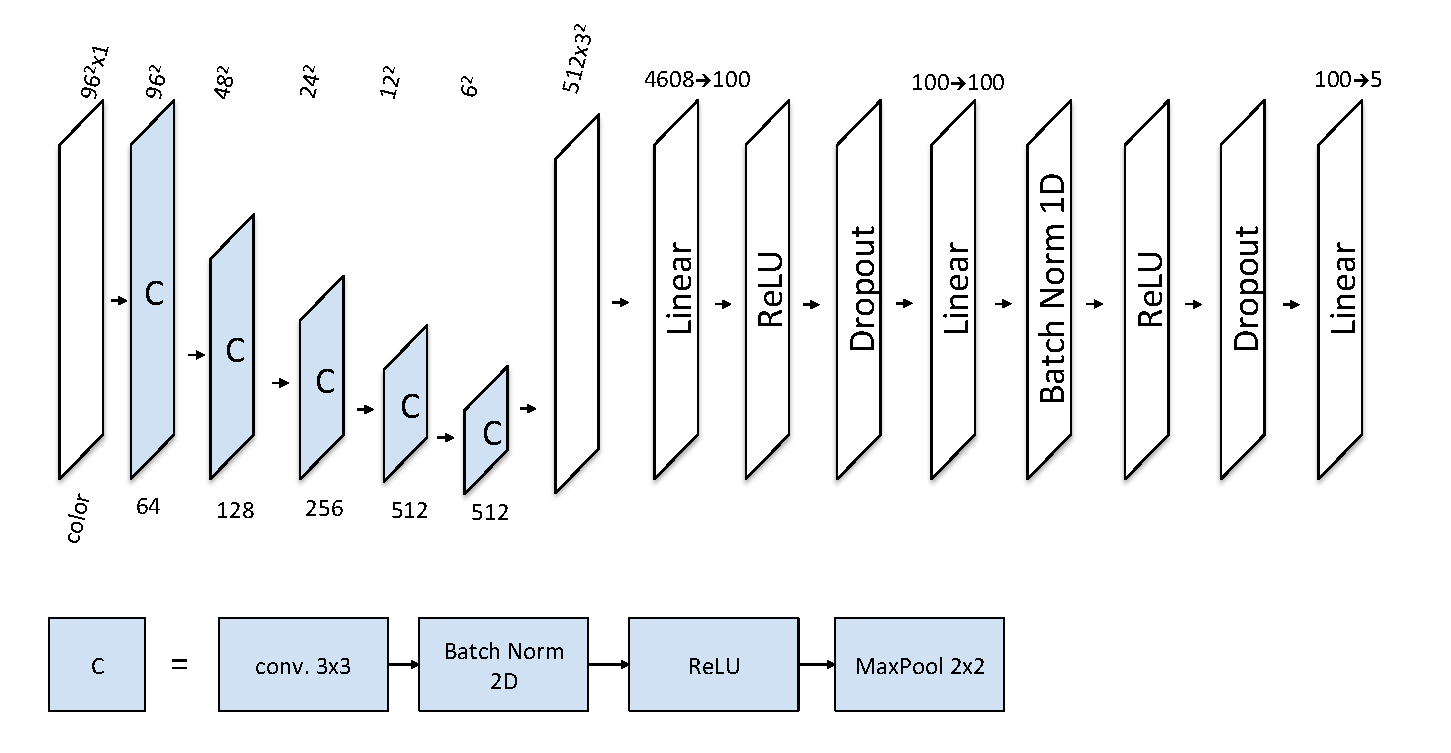
\includegraphics[width=1.0\columnwidth]{./assets/vgg08_diagram.pdf}
\caption{Architecture of VGG08 Batch Norm Classifier}
\label{fig:VGG_DAIGRAM}
\end{figure}

%%%% BEGIN NEW STUFF %%%%
The first experiment done for a dataset is to train a classifier with data that is from the same domain as the test set.  In NORB, this is using the real photographs for training and in ShapeNet, it is the highest sample count Mitsuba rendered images. %Note that for our experiments we use a single lighting condition for both test and training data to simplify experimental setup. A synthetic g-buffer is constructed using Mitsuba for each image in the training set at the target resolution.

This establishes a target classifier accuracy to be used for measuring the induced accuracy of using the training data created by the rendering methods used in this work. Next, we conduct multiple experiments by varying rendering parameters and measuring their quantitative impact on classifier performance.

Next, we use renders that use no shading by taking the albedo maps of each image generated in the g-buffer and using this to train our dataset. We then test this against our baseline generated in the first experiment and compare the results. The output images can be seen in figure \ref{fig:GBUFFER_ALBEDO}.

\begin{figure}[h!]
\centering
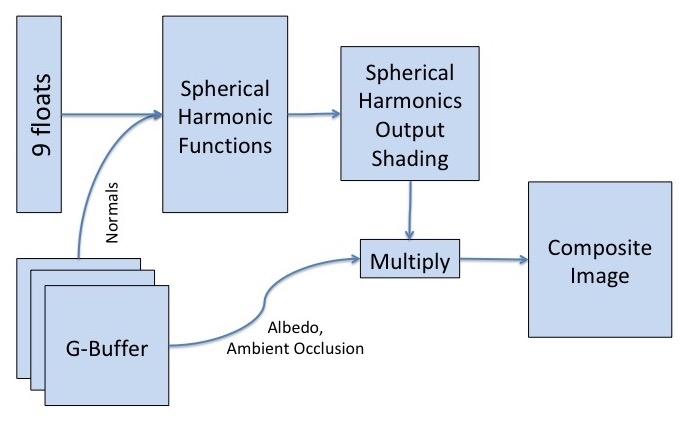
\includegraphics[width=1.0\columnwidth]{./assets/SH_model.jpg}
\caption{Spherical Harmonics network architecture.}
\label{fig:SHN}
\end{figure}

\begin{figure}[h!]
\centering
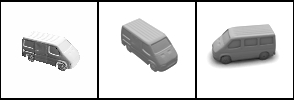
\includegraphics[width=1.0\columnwidth]{./assets/sh-comp-onerow.png}
\caption{Left: Learned SH. Middle: SH x Albedo. Right: SH x Albedo x Ambient Occlusion.}
\label{fig:SHComparison}
\end{figure}
The next step beyond albedo-only rendering is shading the models in the image, but not rendering shadows. In order to do this, we learn the shading using the learnable spherical harmonics module, as seen in figure \ref{fig:SHN}.  We then take these simple shaded renderings and composite them with ambient occlusion (AO) present in the g-buffer as an approximation of lighting condition independent shadowing. An example output image can be seen in figure \ref{fig:SHComparison}. As this is the first experiment that uses shadows, this experiment determines whether or not shadows are important in image classification.

\begin{figure}[h!]
\centering
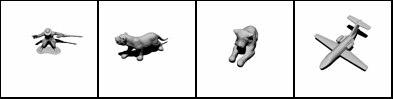
\includegraphics[width=1.0\columnwidth]{./assets/2bounce_small.png}
\caption{Two Bounce Rendering.  Note that it is the equivalent to a shadow mapped scene and differs from the AO composited scenes by the sharpness of the shadows. This is due to the scene using a single directional light.}
\label{fig:2BOUNCE}
\end{figure}
While AO makes a good, fast approximation of shadows, they are not very realistic. Therefore, we next test more realistic shadows. We wish to measure the impact of inter-reflections and global illumination in a later experiment, and so we limit the renderer to do 2-bounce raytracing with a directional light. This allows us to create very hard shadows, as seen in figure \ref{fig:2BOUNCE}.

\begin{figure}[h!]
\centering
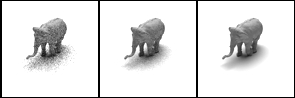
\includegraphics[width=1.0\columnwidth]{./assets/mitsuba-onerow.png}
\caption{
Mitsuba renders at different sample counts. Left: 1 sample per pixel.  Middle: 4.  Right: 128.}
\label{fig:differentsamplesraw}
\end{figure}
Finally, we use a full (GI) renderer to simulate a realistic scene. Using our renderer, this is the closest we can get to the baseline data. As noted earlier, the GI renderer we use, Mitsuba, is a Monte-Carlo raytrace-based renderer, and therefore allowing for more samples-per-pixel will produce a more realistic image. However, as a drawback, higher sample counts take linearly more time to render. 
%TODO: should we add more background about render times (e.g. "our low-sample count images took 1 second to render, high sample count took 100, blah blah...")? 
We test on three different sample counts for each of our datasets to determine how much is gained from using higher values. The difference in sample counts can be seen in figure \ref{fig:differentsamplesraw}.

\begin{figure}[h!]
\centering
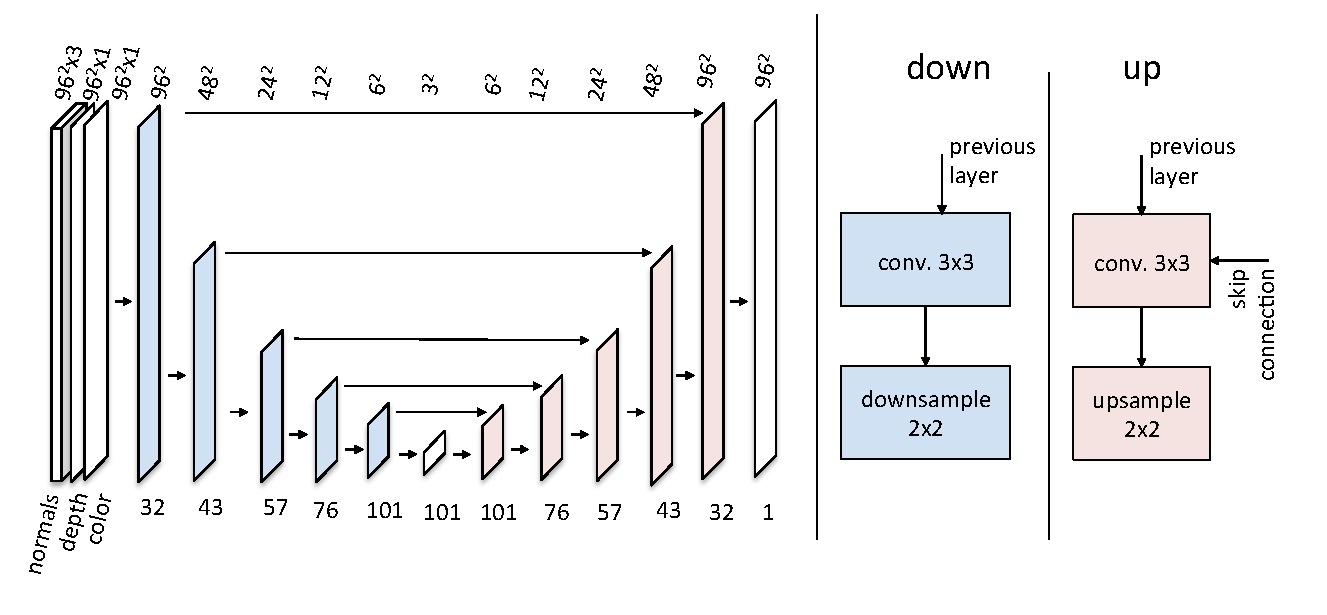
\includegraphics[width=1.0\columnwidth]{./assets/denoiser_diagram.pdf}
\caption{Architecture of Denoising Model}
\label{fig:denoise}
\end{figure}
Given that the low sample GI renders take far less time than the high sample renders, we next experiment to see if the lower sample count images can be denoised using a simplified version of the denoising auto-encoder with skip connections inspired by \cite{Chaitanya:2017:IRM:3072959.3073601}. %We modify this auto-encoder to remove the recurrent portion of the proposed architecture, as we train using static images rather than animated sequences. 
The network architecture is shown in \ref{fig:denoise}. %For this network, we use the Structured Similarity (SSIM) loss function \cite{Wang04imagequality}, a loss function that has proven to be useful for both image-compression measurement and also image comparison. 
%TODO: do we need the long explanation in the paper...?
%See \cite{DBLP:journals/corr/ZhangSYSLJF16} and \cite{DBLP:journals/corr/ZhaoGFK15} for details. 
This denoising process takes milliseconds on the modern GPU, which is a far smaller cost than rendering the high-sample GI renders.

%%%% END NEW STUFF %%%%

%%%%%%%%%%%%%%%%%%%%%%%%%%%%%%%%%%%%%%%%%%%%%%%%%%%%%%%%%%%%%%%%%%%%%%%%%%%%%%%%%%%%%%%%%%%%%%%%%%%%%%%%%%%%
\subsection{Train on GAN Images}
%%%%%%%%%%%%%%%%%%%%%%%%%%%%%%%%%%%%%%%%%%%%%%%%%%%%%%%%%%%%%%%%%%%%%%%%%%%%%%%%%%%%%%%%%%%%%%%%%%%%%%%%%%%%


Another synthetic data generation technique that we explored involved the use of Generative Adversarial Networks (GANs) \cite{2014arXiv1409.7495G}.  We use a GAN architecture inspired by \cite{DBLP:journals/corr/ShrivastavaPTSW16} and \cite{Bousmalis2016UnsupervisedPD}. This work differs from \cite{Bousmalis2016UnsupervisedPD} and \cite{DBLP:journals/corr/ShrivastavaPTSW16} by conditioning on a g-buffer and rendered images with and without the presence of sampling noise. Furthermore, this work doesn't require masking the input images or using local loss functions. This is due to an interesting property of our rendering architecture where by conditioning the generative model on a static g-buffer, and by ensuring that the shading function is dependent on geometry normals (which are not modified by the generative model and is physically motivated by the rendering equation) 
%It has normals as part of the input and shading is highly dependent upon them and they are static during the entire training cycle.
prevents the need for a local loss function and eliminates the problem of a GAN altering the labels of the objects being rendered.
%We modified the SimGAN method for our experiments by removing the local loss function and changing the model architecture of both the refiner and discriminator.  But most importantly, we changed the training and test data domains.  Where SimGAN used synthetic image pixels as input, we pass in image pixels as well a g-buffer \tompson{I took out 'parts' of a g-buffer. That it's a sub-set is an implementation detail}. Specifically, we pass in the normal data and depth buffers along with a rendered image.  
%\tompson{The above paragraph looks way too much like you've just copied their stuff and modified it. This is even more true when you read through the last section where you also took someone else's method and modified it. Here's what I propose. Go through those 2 sections and state something like: "We propose an architecture inspired by [X]. We train a model bla bla bla, to do bla bla bla. Unlike [X] our model is bla." Without trying to take credit for their work, make sure you don't make it seem like you just keep using other people's ideas and don't draw attention to the fact that you're just using existing methods. This requires careful language but I assure you everyone does it.}
%As there is a pre-training step where we run the the self regularization loss against the generator for a number of steps, this ends up pre-training the network to denoise the input image and learn shading.  Then during regular adversarial training this loss helps constrain the shading from drastically changing.  This is also actually a byproduct of the fact that the refiner network is not operating on pixels.
%\tompson{I tried to spice up the last paragraph. I think it's important. But it needs more work.}
%Additionally, in \cite{DBLP:journals/corr/ShrivastavaPTSW16} the input rendered images didn't incorporate global illumination and were farther from real data than our dataset. This means they have more room for improvement in their dataset than in ours. \tompson{Stop using "ours" and "they" it's to informal. "this work" and [X] is the proper way to phrase this. Please go through the whole paper and fix this. Also, I don't know what you mean by this last sentence. The fact that they don't condition on GI is not a BAD thing.}
%Then, the regularization loss is a way to learn the shading just as in the denoising methods.
The GAN architecture we employed was the following:  
The generative network was the same model used for denoising shown in figure \ref{fig:denoise}.  The inputs were normals, depth and either the low, medium and high sample global illumination rendered image. Albedo was used for only ShapeNet data based experiments. The regularization loss was SSIM.

Pre-training the generative network against the high sample Mitsuba rendering before starting adversarial training trained a partially differentiable renderer that learned to denoise and shade the scene conditioned on the g-buffer and image input. Unlike in \cite{DBLP:journals/corr/ShrivastavaPTSW16}, our conditional data distribution is visually very similar to the target generated distribution. As such, we propose a more principled way to validate the performance of the GAN during training (the proposed method in \cite{DBLP:journals/corr/ShrivastavaPTSW16} was to ``visually inspect'' the GAN output and early-stop training when, the output visually resembled the target dataset). To choose a GAN to generate training data we train a classifier on real training and validation data.  No test data is used in testing or training this classifier.  We will call this a clean classifier. For every saved GAN model, we run the synthetic training data through it and establish how well the clean classifier can classify the refined images. We use the classification accuracy to rank the GAN. Take the top 10 GAN refiner models that were ranked from clean classifier and for each one train a classifier on the full dataset. For using multiple GAN models (described below) we take the set of top 10 ranked refiners from the clean classifier and train a classifier with a subset of the refiners synthesizing a new expanded dataset for 200 epochs.

The expanded dataset is created by the following method: Create a new empty training set. For each generative model in the set of refiners; refine each image in the original full training set and append it to the new training set. The new dataset is comprised of $D * N$ images where $N$ is the number of refiners and $D$ is the dataset size.
This effectively generates $N$ copies of the training data where each copy is unique and without the computational overhead of a full render to synthesize the images.

Taking the top 10 models ranked by our method, some outperform just using or denoising the input image.  This method of choosing a GAN allows for choosing a model that outputs non-photorealistic images and represents a principled way to choose models independent from the realism of their generated input.  When evaluating performance of using a single GAN, we took each saved GAN and trained a classifier.  We repeated this three times and then kept the top performing model. For every sample count we found a GAN that could outperform directly training on the original image or denoising it.

% \begin{figure}[h!]
% \centering
% 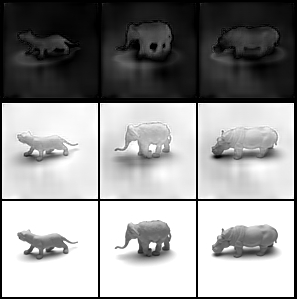
\includegraphics[width=1.0\columnwidth]{./assets/128sampleGANComparison_75_26.png}
% \caption{Bottom: 128 sample Mitsuba passed into GAN, Middle: Output of refiner.  Top: Absolute value difference between full sample the rendered image and the refined image. This particular GAN seems to have brightened up the object albedo and dramatically expanded the shadows.  The performance of using the output from this refiner was 75.26\%. and training directly off of the 128 sample target achieved 74.84\%.}
% \label{fig:GAN_128}
% \end{figure}

\begin{figure}[h!]
\centering
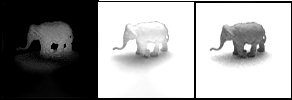
\includegraphics[width=1.0\columnwidth]{./assets/4sampleGAN-onerow.png}
\caption{Right: 4 sample Mitsuba image passed into GAN, Middle: Output of refiner.  Left: Absolute value difference between the full sample rendered image and the refined image. Notice that the image is no longer photo-realistic.}
\label{fig:GAN_4}
\end{figure}

% \begin{figure}[h!]
% \centering
% 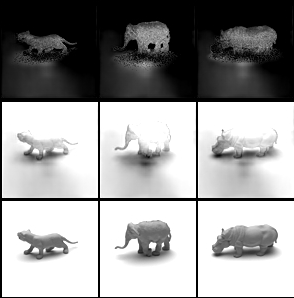
\includegraphics[width=1.0\columnwidth]{./assets/1sampleGANComparison_72_84.png}
% \caption{Bottom: 1 sample Mitsuba image passed into GAN, Middle: Output of refiner.  Top: Absolute value difference between the full sampled rendered image and the refined image. This particular GAN seems to have brightened up the object albedo so much that it erased the top parts of the objects. It has denoised it and has darkened and expanded the shadows down and to the left.  The performance of using the output from this refiner was 72.84\%. and training directly off of the 1 sample target achieved 57.21\%.  Training off the denoised image achieved 71.48\%.}
% \label{fig:GAN_1}
% \end{figure}
\begin{comment}
\edit{MOVE TO RESULTS: 1 sample input GANs scored 72.84\% versus 71.48\% for denoising the same image. See figure \ref{fig:GAN_1} for more details.  The accuracy of the best 4 sample input GAN was 77.65\% versus 73.56\% when just denoised. This was the biggest improvement the GANs achieved versus denoising. See figure \ref{fig:GAN_4} for more details.  With the 128 sample input GAN the performance improved to 75.26\% from 74.84\%. See figure \ref{fig:GAN_128} for more details.}
\end{comment}
\subsubsection{Training using multiple GANs} \label{sec:multigans}
The next experiment is a little different from the rest, as more training data is used and is therefore not quite as comparable.  However, the amount of training data which that would have to be generated in a GI renderer remains the same.  The major change is that the use of the top ten ranked GAN models to create multiple refined version of the data.

The new dataset is an aggregation of the different refined datasets.  The costly pre-rendering of the input images is not changed and the run-time rendering refinement is longer but insignificant compared to GI rendering time.  In our experiments, it took a minute longer to generate 10 times as much data by running the dataset through ten GANS on an NVIDIA Titan X Maxwell GPU. %Even better, the GANs are already there from the training phase and the ranking is already being done. 
The added time for using this method is negligible except for extra time required to train on a larger dataset. This ensemble of GANs is another method in this work that distinguishes it from \cite{Bousmalis2016UnsupervisedPD}.

\begin{comment}
\edit{MOVE TO RESULTS: The resulting performance was significantly better than the best quality GI render, denoising or single GAN output.  The best multi-GAN performance for 1 sample data was 85.23\% using 4 GANs.  For 4-sample data, the best performance came from using 7 GANs and scored 84.37\%. This is close to reducing the error between the best GI rendering and real data by half. Using 128-samples data 7 GANs scored 87.33\%. This reduced the difference between training on real data and the best rendering method by more than half!

In other words, using 128-sample GI rendering is 78.77\% as effective as using real data\footnote{74.84 is 78.77\% of 95.01}.  When you use this measure, a single GAN can boost the effectiveness of synthetic data to 80.01\% of real data.  When an ensemble of GANS is used the synthetic data generated is 91.92\% as effective as real data.
%We have found that you can use a lower sample count image and boost it with a the byproducts of GAN training and reduce the gap between the most realistic rendering methods and real data by half, and slightly more so if you use a high sample count render.  Furthermore, because it is using the byproducts of normal GAN training, it is not more expensive to create the models for this method. The differences in computation are the up front dataset generation from the output of multiple GAN models and having to train on a larger dataset.\\

It is easy to see why this method works. We are creating a more diverse training dataset that has already been tested to be close to the domain of the real dataset.  However, there are diminishing returns.  Adding any more than 8 GANS did not result in better performance.  That may have to do with having a highly weighted regularization loss which prevented the GAN's refined images from deviating too far from the original rendering.  
}
\end{comment}
\section{Results}
We now examine the results from our previous experiments. As the patterns in results between the NORB and ShapeNet datasets were very similar, we will first detail the NORB results, and then use the ShapeNet results to validate these findings.
\begin{table}[]
\centering
\begin{tabular}{|l|r|r|}
\hline
\multicolumn{1}{|c|}{\textbf{Input}}
& \multicolumn{1}{r|}{\textbf{Accuracy}}
& \multicolumn{1}{r|}{\textbf{Baseline \%}} \\ \hline
Albedo Only 				&53.26\%	& 56.06\%	\\
Learned SH Shading			&53.06\%	& 55.85\%	\\
SH Shading + AO				&60.89\%    & 64.09\%   \\
2 Bounce (Direct Lighting)	&66.49\%	& 69.98\%   \\
\textbf{Real Images}		& 95.01\%	& 100.00\%	\\ \hline
\multicolumn{3}{|c|}{\textbf{NORB Performance of Basic Rendering Methods}}	\\ \hline
\end{tabular}

\caption{Performance of real-time (rasterization-based) rendering methods on the NORB dataset. Accuracy is the classification accuracy of the method, and Baseline \% (TODO: rename this?) is how good the method was compared to the baseline render.}
%Albedo Only is passing in the albedo map (see figure \ref{fig:GBUFFER_ALBEDO}). Learned SH Shading is unshadowed shading. SH Shading + AO is unshadowed shading with AO composited with the result. See section \ref{sec:learned_sh} for more detail. 2 Bounce (Direct Lighting) is a shading plus shadowing that is described in section \ref{sec:2bounce}. $\Delta$ vs Real has two numbers: the left is the difference in accuracy from the best result of each method compared to using real data, and the right is the percentage of the real data trained classifier's accuracy that the method achieves.  100\% would mean that the method would have achieved 95.01\% accuracy when training a classifier. Data augmentation was used in all of the above experiments except Real Images. \tompson{Caption is way too big. Move the content here (description of each experiment) to the main body of text.}} 
\label{table:tblnonGI}
\end{table}
\subsection{NORB Results}
The results for the NORB dataset are shown in table \ref{table:tblnonGI}. Albedo Only (unshaded renders) yielded only 53.26\% accuracy. This tells us that while the shape is helpful in classifying an object (compare 53.26\% to 20\% from randomly guessing), it is not nearly enough information to be consistently accurate. This is also the case for the learned SH shading, which scored slightly under the unshaded renders at 53.06\%. We can see that in this case, the fake shading was no more helpful than no shading at all.

We observe slight improvements once shadows are added. AO, our first approximation to shadows, scored at 60.89\% accuracy, a significant jump from renders without shadows. Then, once we improved the quality of shadows with the 2-bounce rendering method, we saw another significant jump to 66.89\% accuracy. However, this is still far less than our target baseline.

\begin{table}[]
\centering
\begin{tabular}{|l|r|r|r|r|}
\hline
\multicolumn{1}{|c|}{\textbf{Input}}
& \multicolumn{1}{c|}{\textbf{Low}}
& \multicolumn{1}{c|}{\textbf{Medium}}
& \multicolumn{1}{c|}{\textbf{High}}
& \multicolumn{1}{c|}{\textbf{Baseline}} \\ \hline
Mitsuba& 64.44\%	& 73.13\%	& 74.74\%	& 78.67\% \\
Denoised& 71.48\%	& 73.56\%	& N/A 		& 77.42\%	\\
GAN& 72.84\%	& 77.65\% 	& 75.26\%	& 81.73\%	\\
Ensemble& 85.23\%	& 84.37\% 	& 87.33\% 	& 91.92\%		\\ \hline
\multicolumn{5}{|c|}{\textbf{Performance of GI Rendered Refined Images}}	\\ \hline
\end{tabular}
\caption{Comparison of GI Rendered Refined Image Performance. The GAN output refers to if only one GAN was used to refine the dataset or if the dataset was expanded by multiple GANs.}
%\caption{Comparison of GI Rendered Refined Image Performance. The GAN output refers to if only one GAN was used to refine the dataset or if the dataset was expanded by multiple GANs\tompson{What GAN output? This is the first time your mentioning GANs. Never, ever, ever, ever (times infinity + 1) show results for a term, model, experiment, etc without first describing it. For this reason, I would move this table WAY down a few pages on.}. $\Delta$ \tompson{IMO, I find this notation confusing. "Performance loss" would be a better column heading.} vs Real has two numbers \tompson{Yes, this is confusing. Pick one of these to show (it's redundant to have both). Simple is better.}. The left is the difference in accuracy from the best result of each method compared to using real data (Real achieved \textbf{95.01\%}). See section \ref{sec:gans} for further details.  The second number is the percentage of the real data trained classifier's accuracy that the method achieves.  100\% would mean that the method would have achieved 95.01\% accuracy when training a classifier. See section \ref{sec:multigans} for more details \tompson{Rule of thumb: a reader should have already read all information they need to understand your results}. Bold values represent values that are better than the accuracy of the best quality GI rendering (128 Sample Mitsuba) \tompson{Remove the bold highlighting.}. Data augmentation was used for the Mitsuba experiments. \tompson{caption is too long. Move some content into body text.}}
\label{table:tblallrefined}
\end{table}

We next observe the results of the more advanced techniques, such as using GI rendering at a high sample count, denoising a low sample count GI rendering, and learning to render using GANs. These results can be observed in table \ref{table:tblallrefined}. While noisy (low sample) GI renders had poor performance, ranking close to the 2-bounce condition we observed earlier, the highest sample GI render achieved 74.74\% accuracy, almost 10\% higher. However, the medium sample count renders performed almost as well as the high sample count renders, demonstrating that beyond a certain quality threshold, the increase in accuracy becomes marginal. 

We can further close the gap between the high sample count renders and the lower sample count renders with the denoising auto-encoder, which brought the 1 sample images to 71.48\% and the 4 sample images to 73.56\% accuracy, less than 1\% difference to the 128 sample render. We can therefore conclude that images could be rendered much faster at low samples, processed with a denoising auto-encoder, and achieve very comparable classification accuracies with a much lower render time.

Finally, we can see that the images generated using the GANs detailed above had a better performance than any other result. With a single GAN, we achieve 75.26\% classification accuracy, which is only a slight increase over the best GI render results. However, with an ensemble of GANs, we were able to achieve an accuracy of 87.33\%, over 90\% of what one can achieve training with real photographic data.
%Learned SH Shading is unshadowed shading. SH Shading + AO is unshadowed shading with AO composited with the result. See section \ref{sec:learned_sh} for more detail. 2 Bounce (Direct Lighting) is a shading plus shadowing that is described in section \ref{sec:2bounce}. $\Delta$ vs Real has two numbers: the left is the difference in accuracy from the best result of each method compared to using real data, and the right is the percentage of the real data trained classifier's accuracy that the method achieves.  100\% would mean that the method would have achieved 95.01\% accuracy when training a classifier. Data augmentation was used in all of the above experiments except Real Images. 
\subsection{ShapeNet Results}

\begin{table}[]
\centering
\begin{tabular}{|l|r|r|}
\hline
\multicolumn{1}{|c|}{\textbf{Input}}
& \multicolumn{1}{r|}{\textbf{Accuracy}}
& \multicolumn{1}{r|}{\textbf{Baseline \%}} \\ \hline
Albedo Only 				&44.44\%	& 52.91\%	\\
Learned SH Shading			&47.80\%	& 56.91\%	\\
%SH Shading + AO				&60.89\%    & 34.12 / 64.09\%   \\
2 Bounce (Direct Lighting)	&70.86\%	& 84.37\%   \\
\textbf{1024 Sample Renderings}		& 83.99\%	& 100.00\%	\\ \hline
\multicolumn{3}{|c|}{\textbf{ShapeNet Performance of Basic Rendering Methods}}	\\ \hline
\end{tabular}
\caption{Performance of real-time (rasterization-based) rendering methods on the ShapeNet dataset.}
\label{table:tblnonGI_sn}
\end{table}

\begin{table}[]
\centering
\begin{tabular}{|l|r|r|r|}
\hline
\multicolumn{1}{|c|}{\textbf{Input}}
& \multicolumn{1}{c|}{\textbf{Low}}
& \multicolumn{1}{c|}{\textbf{Medium}}
%& \multicolumn{1}{c|}{\textbf{128 Sample}}
& \multicolumn{1}{c|}{\textbf{Baseline \%}} \\ \hline
Mitsuba		& 81.68\%	& 82.30\%	& 97.99\% \\
Denoised	& 78.06\%	& 79.12\%	& 96.25\%	\\
GAN	& 83.48\%	& 83.59\%	& \textbf{99.52\%}	\\
Ensemble& 86.48\%	& 86.65\% 	& \textbf{103.17\%}		\\ \hline
\multicolumn{4}{|c|}{\textbf{Performance of GI Rendered Refined Images}}	\\ \hline
\end{tabular}
\caption{Scores using the ShapeNet dataset. Note that the Multiple GAN method performs better than the highest sample render.
%Data augmentation was not used for the experiments listed above.
}
\label{table:tblallrefined_sn}
\end{table}

The ShapeNet results follow very similar patterns to the NORB dataset, as seen in table \ref{table:tblnonGI_sn}. We can see that with the unshaded or learned SH shading models, the classification accuracies are very poor, approximately half of our baseline. Once we move to 2-bounce lighting with shadows, this becomes much closer. We can account for the relatively larger jump in performance when adding shadows compared to NORB because the lighting conditions between the 2-bounce render for ShapeNet were much more similar to the target renders than in the case with the NORB 2-bounce renders and their target. %TODO: this last sentence is kind of a run-on.. it got away from me!

Similarly, due to the nearly identical lighting conditions, we can see in table \ref{table:tblallrefined_sn}, the lower sample renders performed nearly as well as the 1024 sample renders that were used as the baseline. Interestingly, the denoiser reduced classification accuracy. This suggests that the lower sample renders were so similar to the baseline, that even the auto-encoder that attempted to remove noise added artifacts that reduced performance. % TODO: Kris check this, I'm not 100% sure it's right

However, where we see the best performance is when we render with GANs, much like NORB. With a single GAN, we achieve 83.59\% classification accuracy, or 99.52\% of our baseline. When we used an ensemble of GANs, we achieve 86.65\% accuracy, which is even more accurate than our baseline. This means that the GAN-rendered models are as good or better for image classification than the photorealistic, 1024-sample GI renders.

%%%%%%%%%%%%%%%%%%%%%%%%%%%%%%%%%%%%%%%%%%%%%%%%%%%%%%%%%%%%%%%%%%%%%%%%%%%%%%%%%%%%%%%%%%%%%%%%%%%%%%%%%%%%
%%%%%%%%%%%%%%%%%%%%%%%%%%%%%%%%%%%%%%%%%%%%%%%%%%%%%%%%%%%%%%%%%%%%%%%%%%%%%%%%%%%%%%%%%%%%%%%%%%%%%%%%%%%%
\section{Conclusion}

By constructing a novel dataset consisting of synthetic and real images with extremely high levels of geometry correspondence, we are able to directly compare various image synthesis techniques and their impact on domain-adaptation. We do so by measuring the domain-transfer classification accuracy of a multi-class image classifier as a proxy measure for ``image-realism'' as perceived by a Convolutional Network classifier architecture.  We have shown that diffuse shading alone gives similar performance to a simple silhouette image, and that shadows are important for domain transfer.  Most importantly, we proposed two methods to approximate the effectiveness of offline global-illumination rendering, and whose domain adaptation performance actually exceeds it through the use of a learned shading function. The two learned methods optimized for image statistics that are not captured in standard rendering methods which do not take into account the discriminative capacity of convolutional networks. \edit{TODO: revise this previous sentence.} Furthermore, we have also shown that by using an ensemble of GAN models you can beat GI simulation by a significant margin and approach the performance of using real data.
\begin{comment}
\subsection{Future Work}

Because the multiple GAN training model has shown the most promise, an interesting area to research next would be to predict ensembles able produce the best datasets before going through the trouble of training them.
In the future, we intend to expand the dataset by re-photographing the objects and capturing a light probe.  That way, we can eliminate the difference in lighting conditions between the real and the fake images and allow the performance of different shading methods to be more accurately measured.
\tompson{Remove this entire section. Explicit "Future work" sections are more or less out of fashion now. If you really want to add this content, add it inline in the body of the paper.}
\end{comment}
\begin{comment}
\begin{itemize}
\item  Learn lighting in real data using SH network and using unsupervised adversarial training with unlabeled real images... with a single lighting condition.
\item Do 2 bounce lighting training but composite AO.  This is closer to modern game engines that calculate SSAO.
\item Do 3 bounce lighting. Some game engines can do an extra bounce.  Also cheaper.  (NEW PAPER/OR CATEGORY IN THIS PAPER: Take 2 and 3 bounce pairs and learn the 3rd bounce)
\item Do GAN on 2 bounce and 3 bounce lighting to see if it gets near the more expensive methods.
\end{itemize}
\end{comment}
\begin{comment}
\begin{table}[]
\centering
\label{tblallrefined}
\begin{tabular}{|l|r|r|r|r|}
\hline
\multicolumn{1}{|c|}{\textbf{Input}} & \multicolumn{1}{c|}{\textbf{1 Sample}} & \multicolumn{1}{c|}{\textbf{4 Samples}} & \multicolumn{1}{c|}{\textbf{128 Samples}} & \multicolumn{1}{c|}{\textbf{A.O.}} \\ \hline
Mitsuba Output Image                 & 57.21\%                                & 72.89\%                                 & 74.84\%                                   & 58.25\%                                \\
Denoised Images                     & 71.48\%                                & 73.56\%                                 & N/A                                       & N/A                                \\
Single GAN Output                     & 59.20\%                                & 70.40\%                                 & 76.09\%                                   & 63.51\%                            \\
Multiple GAN Output                  & 78.94\%                                   & 84.37\%                                 & 85.33\%                                   & 74.49\%                            \\ \hline
\multicolumn{5}{|c|}{\textbf{Performance of GI Rendered Refined Images}}                                                                                                                                             \\ \hline
\end{tabular}
\caption{Comparison of GI Rendered Refined Image Performance. AO images are actually the g-buffer occlusion channel multiplied by the g-buffer albedo channel.  The GAN output refers to if only one GAN was used to refine the dataset or if the dataset was expanded by multiple GANs each refining their own copy and then combining them into one larger dataset.  See section \ref{sec:gans} for further details.}
\end{table}

\begin{table}[]
\centering
\label{tblnonGI}
\begin{tabular}{|l|r|}
\hline
\multicolumn{1}{|c|}{\textbf{Input}} & \multicolumn{1}{c|}{\textbf{Accuracy}} \\ \hline
Albedo Only                          & 46.20\%                                \\
Learned SH Shading                   & 48.52\%                                \\
SH Shading + AO                      & 55.80\%                                \\
Shadow Mapped (2 Bounce)              & 55.78\%                                \\ 
\textbf{Real Images}                           & \textbf{95.01}\%                                \\ \hline
\multicolumn{2}{|c|}{\textbf{Performance Of Non GI Rendering}}                \\ \hline
\end{tabular}
\caption{Non Global Illumination Based Rendering Performance. Albedo Only is passing in the albedo map see figure \ref{fig:GBUFFER_ALBEDO}. Learned SH Shading is unshadowed shading and SH Shading + AO is unshadowed shading with the g-buffer occlusion channel multiplied against the result. See section \ref{sec:learned_sh} for more detail. Shadow Mapped (2 Bounce) is a shading plus shadowing that is described in section \ref{sec:2bounce}. } 
\end{table}


\subsection{Ambient Occlusion Conclusions}
\subsubsection{Varying Lighting}
Learning Spherical Harmonics certainly works for a single lighting condition.  But a problem we forsee is that the test data is under six different lighting conditions and we might want to learn either multiple lighting conditions or have the network be able to learn an arbitrary number of lighting conditions (no design limit to the number of lighting conditions).  

How do we do this?  Is there a way to have feature map count like convolutions?  Like input of 1x96x96 and output Nx1x96x96?  I think this might work.
\subsubsection{Learning Albedo}
During initial experiments we noticed that if the object albedo was not close the non GAN (we didn't have GANs implemented yet) networks would not do better than random guessing on the test set.  However once albedo was approximately the same (in our particular case a medium gray) test performance shot up.  Therefore, it was decided that albedo should be a learnable parameter so object color could be optimized for learning.

The question that arises is should albedo be per object, per material or per pixel?  We will have to try all three.  My guess per object and per material will the most interpretable but per pixel might be the best(or might overfit quickly).

\subsubsection{Shadows and Ambient Occlusion}
While exploring ambient occlusion based images for training we noticed that objects that had minimal shadow, such as people, cars and trucks, in the real data classified well when using AO images.  People objects have the toy base which mostly covers the shadow and cars are low enough to the ground that the shadow doesn't take a large percentage of the image.  However the objects that cast relatively large shadows such as animals an planes have very poor performance when training with AO rendered images.  Shadows Matter!\\

See Figures \ref{fig:mitsuba-AO} and \ref{fig:mitsuba-AO2} for sample renders.

\end{comment}
\begin{comment}
%Connor says that this was on training data that wasn't centered and put into an 80x80 box
\begin{lstlisting}[language=bash]
%python2 main.py --viz-data --use-visdom --visdom-url=http://172.24.70.20 --visdom-port=8097 --train-type=mcmitsuba --data-dir=datasets/mitsuba/large/path/ --lr=1e-5 --epochs=100
%
^^^^^^^^^^^^^^^^^^^^^^^^^^^^^^^^^^^^^^^^^^^^^^^^^^^^^^^^^^^^^^^^^^^^^^^
^^^^^^^^^^^^^^^^^^^^^^^^^^^^^^^^^^^^^^^^^^^^^^^^^^^^^^^^^^^^^^^^^^^^^^^
Best accuracy was 53.63% in epoch 86
ConfusionMatrix:
[[      73     131     509       4      93]   9.012%	[class: animal]
 [       0     585     225       0       0]   72.222%	[class: people]
 [       9       1     542      51     207]   66.914%	[class: plane]
 [      46      14      96     544     110]   67.160%	[class: truck]
 [      61       5     180     136     428]]  52.840%	[class: car]
 + average row correct: 53.63
 + average rowUcol correct (VOC measure): 37.59%
 + global correct: 53.63%
^^^^^^^^^^^^^^^^^^^^^^^^^^^^^^^^^^^^^^^^^^^^^^^^^^^^^^^^^^^^^^^^^^^^^^^
^^^^^^^^^^^^^^^^^^^^^^^^^^^^^^^^^^^^^^^^^^^^^^^^^^^^^^^^^^^^^^^^^^^^^^^
\end{lstlisting}

\begin{figure}[h!]
\centering
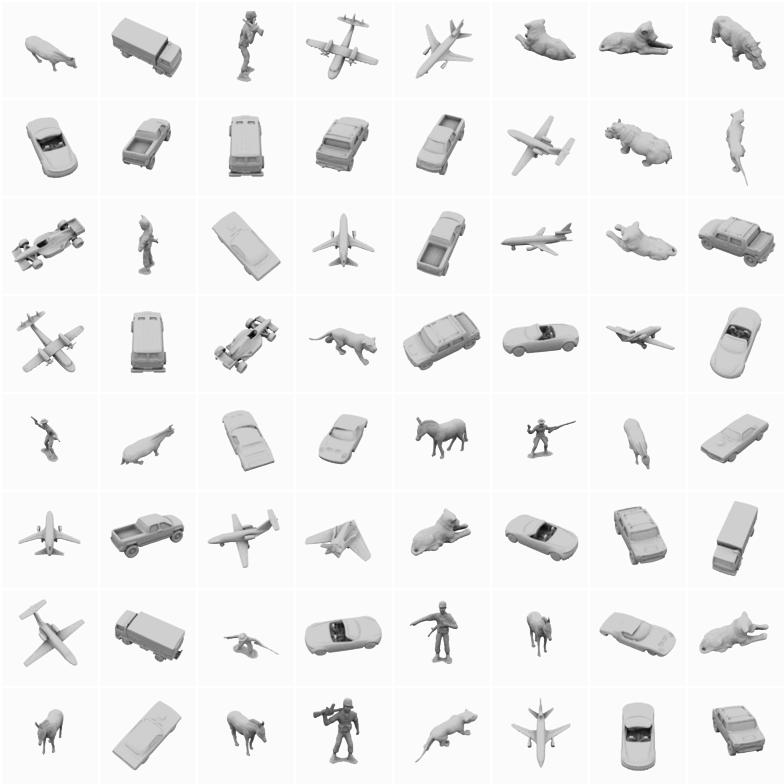
\includegraphics[width=0.8\textwidth]{./assets/mcm-train.png}
\caption{A sample of some of the images generated with Mitsuba using an Ambient Occlusion rendering technique but with a scene lacking a ground plane.}
\label{fig:mitsuba-AO-no-ground}
\end{figure}

In our test we tried using AO to simulate shadows with a relatively short ray length versus a longer ray length.  The difference is that the occlusion calculated was more local and better suited for the environment the test data was photographed in.  We note that here, not only was the accuracy higher than the previous test, but the difference between the highest accuracy label and the lowest accuracy label is much smaller.  The long ray length AO training data only produced a classifier with about 53\% accuracy versus 63\% for a shorter length.  The is approximately the difference between OpenGL and GAN learned shading.  This makes sense in that long ray AO produced a mismatch in the lighting from the test set just like the directional lighting in the OpenGL set.  The shorter ray AO as well as the GAN softened the shadowing which is closer to the test data and as a result they both performed better.\\

%%%%%%%%%%%%%%%%%%%%%%%%%%%%%%%%%%%%%%%%%%%%%%%%%%%%%%%%%%%%%%%%%%%%%%%%%%%%%%%%%%%%%%%%%%%%%%%%%%%%%%%%%%%%
\subsection{Computational Cost}
%%%%%%%%%%%%%%%%%%%%%%%%%%%%%%%%%%%%%%%%%%%%%%%%%%%%%%%%%%%%%%%%%%%%%%%%%%%%%%%%%%%%%%%%%%%%%%%%%%%%%%%%%%%%

Calculating AO properly is expensive and required a global-illumination renderer to sample at the geometry surface and fire rays sampling the hemisphere for any intersections with solid surfaces. However there are techniques that you can use a GPU to approximate AO in real-time.  However the effect of this approximation should be measured.  This is future work.

\end{comment}
\begin{comment}
\begin{lstlisting}[language=bash]
python2 main.py --viz-data --use-visdom --visdom-url=http://172.24.70.20 --visdom-port=8097 --train-type=mcmitsuba --data-dir=datasets/mitsuba/large/path/ --lr=1e-3 --epochs=300 --add-noise

^^^^^^^^^^^^^^^^^^^^^^^^^^^^^^^^^^^^^^^^^^^^^^^^^^^^^^^^^^^^^^^^^^^^^^^
^^^^^^^^^^^^^^^^^^^^^^^^^^^^^^^^^^^^^^^^^^^^^^^^^^^^^^^^^^^^^^^^^^^^^^^
Best accuracy was 63.06% in epoch 141
ConfusionMatrix:
[[     377     218     151      11      53]   46.543%	[class: animal]
 [       7     652     121      12      18]   80.494%	[class: people]
 [      91      31     632      36      20]   78.025%	[class: plane]
 [      96      59      27     535      93]   66.049%	[class: truck]
 [     223      48      20     161     358]]  44.198%	[class: car]
 + average row correct: 63.06
 + average rowUcol correct (VOC measure): 46.12%
 + global correct: 63.06%
^^^^^^^^^^^^^^^^^^^^^^^^^^^^^^^^^^^^^^^^^^^^^^^^^^^^^^^^^^^^^^^^^^^^^^^
^^^^^^^^^^^^^^^^^^^^^^^^^^^^^^^^^^^^^^^^^^^^^^^^^^^^^^^^^^^^^^^^^^^^^^^

\end{lstlisting}

\begin{figure}[h!]
\centering
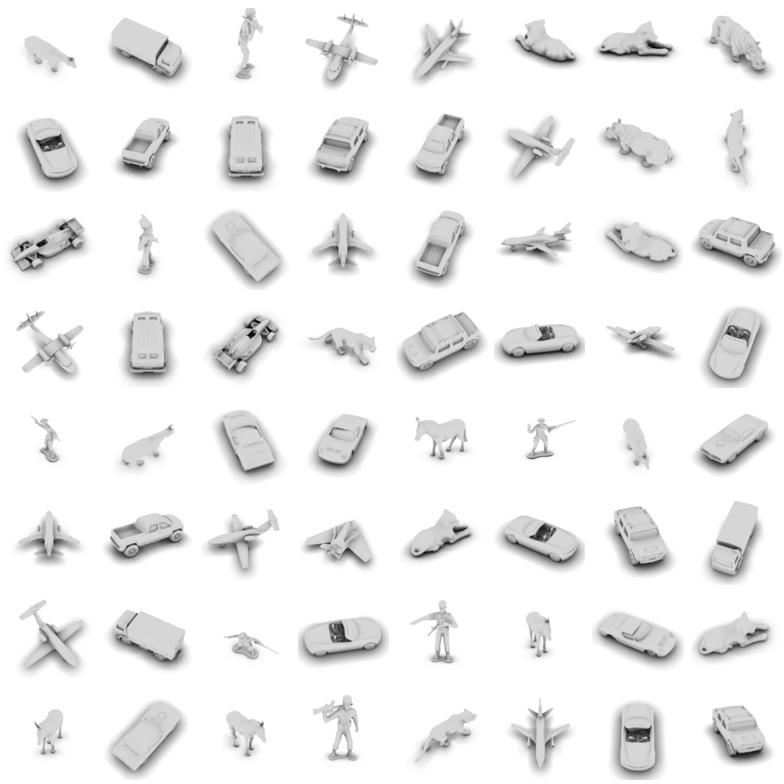
\includegraphics[width=0.8\textwidth]{./assets/mcm-train2.png}
\caption{A sample of some of the images generated with Mitsuba using an Ambient Occlusion rendering technique. Here, a ground plane was introduced to create shadow and the AO ray length was reduced.}
\label{fig:mitsuba-AO2}
\end{figure}
\end{comment}

%%%%%%%%%%%%%%%%%%%%%%%%%%%%%%%%%%%%%%%%%%%%%%%%%%%%%%%%%%%%%%%%%%%%%%%%%%%%%%%%%%%%%%%%%%%%%%%%%%%%%%%%%%%%
%%%%%%%%%%%%%%%%%%%%%%%%%%%%%%%%%%%%%%%%%%%%%%%%%%%%%%%%%%%%%%%%%%%%%%%%%%%%%%%%%%%%%%%%%%%%%%%%%%%%%%%%%%%%

\newpage



%%%%%%%%%%%%%%%%%%%%%%%%%%%%%%%%%%%%%%%%%%%%%%%%%%%%%%%%%%%%%%%%%%%%%%%%%%%%%%%%%%%%%%%%%%%%%%%%%%%%%%%%%%%%
%%%%%%%%%%%%%%%%%%%%%%%%%%%%%%%%%%%%%%%%%%%%%%%%%%%%%%%%%%%%%%%%%%%%%%%%%%%%%%%%%%%%%%%%%%%%%%%%%%%%%%%%%%%%
%%%%%%%%%%%%%%%%%%%%%%%%%%%%%%%%%%%%%%%%%%%%%%%%%%%%%%%%%%%%%%%%%%%%%%%%%%%%%%%%%%%%%%%%%%%%%%%%%%%%%%%%%%%%
%%%%%%%%%%%%%%%%%%%%%%%%%%%%%%%%%%%%%%%%%%%%%%%%%%%%%%%%%%%%%%%%%%%%%%%%%%%%%%%%%%%%%%%%%%%%%%%%%%%%%%%%%%%%
%%%%%%%%%%%%%%%%%%%%%%%%%%%%%%%%%%%%%%%%%%%%%%%%%%%%%%%%%%%%%%%%%%%%%%%%%%%%%%%%%%%%%%%%%%%%%%%%%%%%%%%%%%%%
%%%%%%%%%%%%%%%%%%%%%%%%%%%%%%%%%%%%%%%%%%%%%%%%%%%%%%%%%%%%%%%%%%%%%%%%%%%%%%%%%%%%%%%%%%%%%%%%%%%%%%%%%%%%
%%%%%%%%%%%%%%%%%%%%%%%%%%%%%%%%%%%%%%%%%%%%%%%%%%%%%%%%%%%%%%%%%%%%%%%%%%%%%%%%%%%%%%%%%%%%%%%%%%%%%%%%%%%%
%%%%%%%%%%%%%%%%%%%%%%%%%%%%%%%%%%%%%%%%%%%%%%%%%%%%%%%%%%%%%%%%%%%%%%%%%%%%%%%%%%%%%%%%%%%%%%%%%%%%%%%%%%%%
%%%%%%%%%%%%%%%%%%%%%%%%%%%%%%%%%%%%%%%%%%%%%%%%%%%%%%%%%%%%%%%%%%%%%%%%%%%%%%%%%%%%%%%%%%%%%%%%%%%%%%%%%%%%
%%%%%%%%%%%%%%%%%%%%%%%%%%%%%%%%%%%%%%%%%%%%%%%%%%%%%%%%%%%%%%%%%%%%%%%%%%%%%%%%%%%%%%%%%%%%%%%%%%%%%%%%%%%%
%%%%%%%%%%%%%%%%%%%%%%%%%%%%%%%%%%%%%%%%%%%%%%%%%%%%%%%%%%%%%%%%%%%%%%%%%%%%%%%%%%%%%%%%%%%%%%%%%%%%%%%%%%%%
%%%%%%%%%%%%%%%%%%%%%%%%%%%%%%%%%%%%%%%%%%%%%%%%%%%%%%%%%%%%%%%%%%%%%%%%%%%%%%%%%%%%%%%%%%%%%%%%%%%%%%%%%%%%
%%%%%%%%%%%%%%%%%%%%%%%%%%%%%%%%%%%%%%%%%%%%%%%%%%%%%%%%%%%%%%%%%%%%%%%%%%%%%%%%%%%%%%%%%%%%%%%%%%%%%%%%%%%%
%%%%%%%%%%%%%%%%%%%%%%%%%%%%%%%%%%%%%%%%%%%%%%%%%%%%%%%%%%%%%%%%%%%%%%%%%%%%%%%%%%%%%%%%%%%%%%%%%%%%%%%%%%%%
%%%%%%%%%%%%%%%%%%%%%%%%%%%%%%%%%%%%%%%%%%%%%%%%%%%%%%%%%%%%%%%%%%%%%%%%%%%%%%%%%%%%%%%%%%%%%%%%%%%%%%%%%%%%

\begin{comment}
\section{APPENDIX A - Non-Standard G-Buffer Experiments}
\subsection{Randomized SH Weights Experiment}
The following experiments train a classifier with a generative SH net but this time the loss ignored and the generative net has its parameters randomly set from a uniform distribution.
The classifier is effectively trained with randomly lit objects. Where the lighting is restricted to a smooth function along a sphere's surface.
\begin{enumerate}
\item Per Training Epoch
\begin{enumerate}
\item Randomly set SH weights
\item Iterate through all of the training data which in this case is the normal buffer part of a G-Buffer 
\item Classify generated images.
\item Use loss to update the classifier.
\end{enumerate}
\end{enumerate}

Then use the trained classifier C to classify real test images.\\
Results for 500 epochs
\begin{lstlisting}[language=bash]
%$ python test_sh4_use_random_weights.py --viz-data --visdom-env kris 
%--use-visdom --epochs 500 --lr 1e-3 --data-dir datasets/opengl/small/ --cuda-device 1
%# Using random weights for SH to train classifier.  500 epochs. 
^^^^^^^^^^^^^^^^^^^^^^^^^^^^^^^^^^^^^^^^^^^^^^^^^^^^^^^^^^^^^^^^^^^^^^^
^^^^^^^^^^^^^^^^^^^^^^^^^^^^^^^^^^^^^^^^^^^^^^^^^^^^^^^^^^^^^^^^^^^^^^^
Best accuracy was 46.86% in epoch 424
ConfusionMatrix:
[[     414      92     278      18       8]   51.111%	[class: animal]
 [      39     760      11       0       0]   93.827%	[class: people]
 [      78     110     618       1       3]   76.296%	[class: plane]
 [     160       8     497      18     127]   2.222%	[class: truck]
 [     240       5     463      14      88]]  10.864%	[class: car]
 + average row correct: 46.86
 + average rowUcol correct (VOC measure): 29.36%
 + global correct: 46.86%
^^^^^^^^^^^^^^^^^^^^^^^^^^^^^^^^^^^^^^^^^^^^^^^^^^^^^^^^^^^^^^^^^^^^^^^
^^^^^^^^^^^^^^^^^^^^^^^^^^^^^^^^^^^^^^^^^^^^^^^^^^^^^^^^^^^^^^^^^^^^^^^
\end{lstlisting}
Results for 10,000 epochs
\begin{lstlisting}[language=bash]

%$ python test_sh4_use_random_weights.py --epochs 10000 --lr 1e-3 
%--data-dir datasets/opengl/small/
%# trained with random sh weights per epoch. No loss used to guide it.
^^^^^^^^^^^^^^^^^^^^^^^^^^^^^^^^^^^^^^^^^^^^^^^^^^^^^^^^^^^^^^^^^^^^^^^
^^^^^^^^^^^^^^^^^^^^^^^^^^^^^^^^^^^^^^^^^^^^^^^^^^^^^^^^^^^^^^^^^^^^^^^
Best accuracy was 47.78% in epoch 646
ConfusionMatrix:
[[     554     117      92      47       0]   68.395%   [class: animal]
 [      26     762      13       9       0]   94.074%   [class: people]
 [     205     177     415      13       0]   51.235%   [class: plane]
 [     221       5     373     190      21]   23.457%   [class: truck]
 [     319       7     307     163      14]]  1.728%    [class: car]
 + average row correct: 47.78
 + average rowUcol correct (VOC measure): 29.85%
 + global correct: 47.78%
^^^^^^^^^^^^^^^^^^^^^^^^^^^^^^^^^^^^^^^^^^^^^^^^^^^^^^^^^^^^^^^^^^^^^^^
^^^^^^^^^^^^^^^^^^^^^^^^^^^^^^^^^^^^^^^^^^^^^^^^^^^^^^^^^^^^^^^^^^^^^^^
\end{lstlisting}
Results for 100,000 epochs
\begin{lstlisting}[language=bash]
%$ python test_sh4_use_random_weights.py --epochs 100000 --lr 1e-3 
%--data-dir datasets/opengl/small/ 
%# trained with random sh weights per epoch. No loss used to guide it.
^^^^^^^^^^^^^^^^^^^^^^^^^^^^^^^^^^^^^^^^^^^^^^^^^^^^^^^^^^^^^^^^^^^^^^^
^^^^^^^^^^^^^^^^^^^^^^^^^^^^^^^^^^^^^^^^^^^^^^^^^^^^^^^^^^^^^^^^^^^^^^^
Best accuracy was 49.43% in epoch 1660
ConfusionMatrix:
[[     355      74     271       2     108]   43.827%   [class: animal]
 [      40     717      50       3       0]   88.519%   [class: people]
 [      57      57     601       1      94]   74.198%   [class: plane]
 [      28       0     319      36     427]   4.444%    [class: truck]
 [      53       0     427      37     293]]  36.173%   [class: car]
 + average row correct: 49.43
 + average rowUcol correct (VOC measure): 33.75%
 + global correct: 49.43%
^^^^^^^^^^^^^^^^^^^^^^^^^^^^^^^^^^^^^^^^^^^^^^^^^^^^^^^^^^^^^^^^^^^^^^^
^^^^^^^^^^^^^^^^^^^^^^^^^^^^^^^^^^^^^^^^^^^^^^^^^^^^^^^^^^^^^^^^^^^^^^^
\end{lstlisting}
As you can see the more examples it is shown the better it gets however there are clearly diminishing returns and it seems that it didn't benefit from more than 20,000 epochs so adding any epochs would probably gain nothing in accuracy.
\subsection{Basic OpenGL Directional Lighting and Shadow Mapping}
\begin{figure}[h!]
\centering
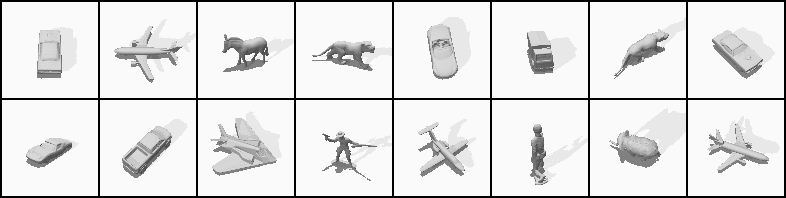
\includegraphics[width=0.95\textwidth]{./assets/dotsynthshadow_training.jpg}
\caption{OpenGL Rendering Example.  Notice the two shadows with varying intensity.}
\label{fig:OGLDOTSYNTH}
\end{figure}
\begin{figure}[h!]
\centering
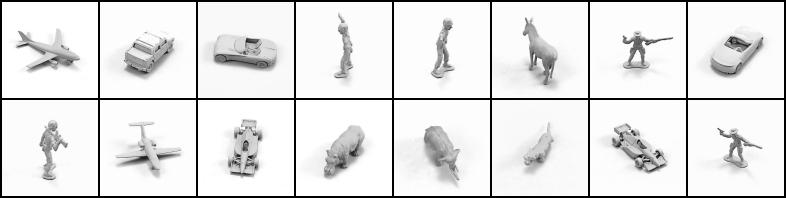
\includegraphics[width=0.95\textwidth]{./assets/TrainDataReal16.png}
\caption{Real NORB Training Data Photographs}
\label{fig:REALTRAIN}
\end{figure}
The most basic rendering was with a simple OpenGL based renderer that had two directional lights of differing intensities.  Shadows were calculated per light.  See Figure \ref{fig:OGLDOTSYNTH} for an example rendering of some training data. Compare it with real training data in Figure \ref{fig:REALTRAIN}.\\
The OpenGL API makes this kind of rendering very efficient on a GPU and thousands of images can be generated per second.  The images created for this test took less than a millisecond to calculate.  The copy down to the CPU and writing to disk slowed everything down to roughly 300 images a second rendered and written to disk on a Titan X (Maxwell). If buffers were shared with CUDA then used directly in training the rendering time would be insignificant.  Because this is the easiest and cheapest method for creating data we will consider it the baseline for comparing the rest of the rendering methods.\\
While this method is cheap it is also not very effective in training a classifier.  See Figure \ref{fig:PLOTOPENGL} to see that we only get around 50\% accuracy when testing on the real NORB test data.
\begin{figure}[h!]
\centering
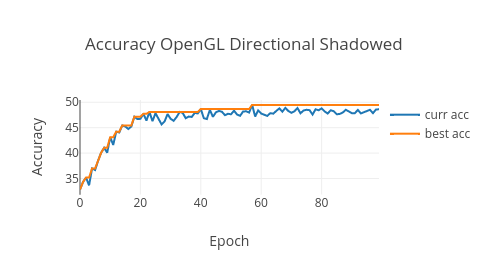
\includegraphics[width=0.95\textwidth]{./assets/OpenGL_DotSynth_Performance.png}
\caption{Accuracy of classifier trained with OpenGL Directional Lighting with Shadows.  It maxed out at 49.48\%.}
\label{fig:PLOTOPENGL}
\end{figure}

\end{comment}
%\begin{lstlisting}[language=bash]
%^^^^^^^^^^^^^^^^^^^^^^^^^^^^^^^^^^^^^^^^^^^^^^^^^^^^^^^^^^^^^^^^^^^^^^^
%^^^^^^^^^^^^^^^^^^^^^^^^^^^^^^^^^^^^^^^^^^^^^^^^^^^^^^^^^^^^^^^^^^^^^^^
%Best accuracy was 49.48% in epoch 58
%ConfusionMatrix:
%[[     685       0       0       9     116]   84.568%	[class: animal]
% [     135     321       0       0     354]   39.630%	[class: people]
% [     354      14       0      28     414]   0.000%	[class: plane]
% [     116       0       0     401     293]   49.506%	[class: truck]
% [     183       0      20      10     597]]  73.704%	[class: car]
% + average row correct: 49.48
% + average rowUcol correct (VOC measure): 31.73%
% + global correct: 49.48%
%^^^^^^^^^^^^^^^^^^^^^^^^^^^^^^^^^^^^^^^^^^^^^^^^^^^^^^^^^^^^^^^^^^^^^^^
%^^^^^^^^^^^^^^^^^^^^^^^^^^^^^^^^^^^^^^^^^^^^^^^^^^^^^^^^^^^^^^^^^^^^^^^
%\end{lstlisting}
%
%\subsection{Training with Global Illumination Renderer}
%The following experiments were conducted using images calculated using Mitsuba with various integrators, such as Direct (Ray Tracing) and Path (Path Tracing).
%\begin{lstlisting}[language=bash]
%$ python main.py --train-type 'trainsynth' --lr 1e-4
%# This is on 48600 direct integrator mitsuba.  10 lighting conditions and 
%# only 1 test lighting condition
%^^^^^^^^^^^^^^^^^^^^^^^^^^^^^^^^^^^^^^^^^^^^^^^^^^^^^^^^^^^^^^^^^^^^^^^
%ConfusionMatrix:
%[[     700      46       7       0      57]   86.420%	[class: animal]
% [       5     724      71       0      10]   89.383%	[class: people]
% [      57       6     704       0      43]   86.914%	[class: plane]
% [      44       0       0     734      32]   90.617%	[class: truck]
% [      16       2      39     401     352]]  43.457%	[class: car]
% + average row correct: 79.36
% + average rowUcol correct (VOC measure): 66.49%
% + global correct: 79.36%
%-----> *** Best model so far.  Saving checkpoint for epoch 28 pct 79.36*** <----
%^^^^^^^^^^^^^^^^^^^^^^^^^^^^^^^^^^^^^^^^^^^^^^^^^^^^^^^^^^^^^^^^^^^^^^^
%
%$ python main.py --train-type 'trainsynth' --lr 5e-6 
%--data-dir datasets/mitsuba/large/path/ --epochs 300
%# This is on 48600 path integrator mitsuba.  10 lighting conditions and only 1 
%# test lighting condition
%^^^^^^^^^^^^^^^^^^^^^^^^^^^^^^^^^^^^^^^^^^^^^^^^^^^^^^^^^^^^^^^^^^^^^^^
%Best accuracy was 74.96% in epoch 169
%ConfusionMatrix:
%[[     616     104      58       0      32]   76.049%   [class: animal]
% [       2     684     124       0       0]   84.444%   [class: people]
% [      10       4     708       8      80]   87.407%   [class: plane]
% [      76       0       8     647      79]   79.877%   [class: truck]
% [     110       0      45     274     381]]  47.037%   [class: car]
% + average row correct: 74.96
% + average rowUcol correct (VOC measure): 60.14%
% + global correct: 74.96%
% 
%$ python main.py --train-type 'genbprop' --lr 1e-4 --epochs 300 --viz-data
%# This is on 51,839 gbuffer(normals).  Test set is 12,960 gbuffer images.  
%# The pretrained model had 90.79% accuracy on real data and was trained from real data.
%^^^^^^^^^^^^^^^^^^^^^^^^^^^^^^^^^^^^^^^^^^^^^^^^^^^^^^^^^^^^^^^^^^^^^^^
%^^^^^^^^^^^^^^^^^^^^^^^^^^^^^^^^^^^^^^^^^^^^^^^^^^^^^^^^^^^^^^^^^^^^^^^
%Best accuracy was 85.06% in epoch 284
%ConfusionMatrix:
%[[    2592       0       0       0       0]   100.000%  [class: animal]
% [       5    2587       0       0       0]   99.807%   [class: people]
% [     161       0    1426      97     908]   55.015%   [class: plane]
% [      16       0       4    2140     432]   82.562%   [class: truck]
% [      14       0      29     270    2279]]  87.924%   [class: car]
% + average row correct: 85.06
% + average rowUcol correct (VOC measure): 75.48%
% + global correct: 85.06%
%^^^^^^^^^^^^^^^^^^^^^^^^^^^^^^^^^^^^^^^^^^^^^^^^^^^^^^^^^^^^^^^^^^^^^^^
%^^^^^^^^^^^^^^^^^^^^^^^^^^^^^^^^^^^^^^^^^^^^^^^^^^^^^^^^^^^^^^^^^^^^^^^
% 
%python main.py --train-type=mcmitsuba --data-dir=datasets/mitsuba/small/path/
%# Trained using combined image, normals, occlusion, and albedo data on 400 synthetic Mitsuba-generated images.
%^^^^^^^^^^^^^^^^^^^^^^^^^^^^^^^^^^^^^^^^^^^^^^^^^^^^^^^^^^^^^^^^^^^^^^^
%^^^^^^^^^^^^^^^^^^^^^^^^^^^^^^^^^^^^^^^^^^^^^^^^^^^^^^^^^^^^^^^^^^^^^^^
%Best accuracy was 74.00% in epoch 49
%ConfusionMatrix:
%[[       8       5       0       7       0]   40.000%	[class: animal]
% [       3      16       0       1       0]   80.000%	[class: people]
% [       1       0      19       0       0]   95.000%	[class: plane]
% [       0       0       2      18       0]   90.000%	[class: truck]
% [       0       0       0       7      13]]  65.000%	[class: car]
% + average row correct: 74.00
% + average rowUcol correct (VOC measure): 60.03%
% + global correct: 74.00%
%^^^^^^^^^^^^^^^^^^^^^^^^^^^^^^^^^^^^^^^^^^^^^^^^^^^^^^^^^^^^^^^^^^^^^^^
%^^^^^^^^^^^^^^^^^^^^^^^^^^^^^^^^^^^^^^^^^^^^^^^^^^^^^^^^^^^^^^^^^^^^^^^
%
% 
%\end{lstlisting}
\begin{comment}
\subsection{Adversarial Training with goal of maximizing classification performance}
G = Generator Network.  Which can be a GBuffer with a Spherical Harmonics or Convolutional Block on top of it.
C = Classifier.  Experiment with architectures.. but start with the one used in the NORB paper.
\subsection{Training method}
G creates rendered synthetic images S.  S is fed into C and C updates its weights but does not send loss to G. After each epoch the real test data S is sent into C and the loss is sent to G to update its weights.  The goal is to only use the misclassification loss to update G.  The goal isn't for G to make images as realistic and as close to S as possible.  Its main goal is to have G produce S that maximizes the performance C learning how to classify R. 

This is a tick - tock pattern where on tick C learns from S and on tock G learns from R fed into C.  Each tick and tock are an "epoch" in the sense that all of the data is passed through once.

\subsection{Adversarial Training using SIMGAN as a baseline}
This has the advantages of being able to use unlabeled data. 
\begin{itemize}
  \item Start with GBuffer.  This might prevent the need for a local adversarial loss.
  \item Also experiment with starting with 
    \begin{itemize}
      \item Directional lighting
      \item AO
      \item Path Traced
      \item Direct Ray Tracing
    \end{itemize}
\end{itemize}
\end{comment}

%
%\subsection{Style Transfer as a data gen technique}
%http://www.creativeai.net/posts/DxEdiP2D74kmkfZrZ/arbitrary-style-transfer-in-real-time-with-adaptive-instance
%
%
%This has the advantage of creating many NPR styles that we can test
%\begin{itemize}
%  \item Start with Pixels of the type:
%    \begin{itemize}
%      \item Directional lighting
%      \item AO
%      \item Path Traced
%      \item Direct Ray Tracing
%    \end{itemize}
%  \item Then use a variety of images to style them and train on them and test performance.
%  \item can we use the loss to update the style????  Maybe. SOMETHING TO TRY.
%  \item this is like a differentiable shader if we can update the style based upon the loss in classification.
%\end{itemize}
%
%\subsection{Train on GBuffer}
%\subsection{Pre-train Classifier on Real Data and make that an adversarial loss for generator}
%\begin{itemize}
%\item What loss should I use to update the generator?
%\item What model should I use for the generator?
%\end{itemize}
%
%\subsection{Learning from Simulated and Unsupervised Images through Adversarial Training}
%For eye gaze tracking they train with synthetic data from the UnityEyes or refined datasets and test on the real data from MPIIGaze.  They don't pre-train of or do any transfer learning.
%\subsection{Experiments}
%\begin{itemize}
%\item Synthetic Data
%\item Synthetic Data x4
%\item Refined Data
%\item Refined Data x4
%\end{itemize}
%
\begin{comment}
\section{APPENDIX B Other Papers}
\subsection{Physically-Based Rendering for Indoor Scene Understanding Using Convolutional Neural Nets}

\subsection{Experiments}
\subsubsection{Terminology}
In the neural network terminology:

\textbf{one epoch} = one forward pass and one backward pass of all the training examples

\textbf{batch size} = the number of training examples in one forward/backward pass. The higher the batch size, the more memory space you'll need.

\textbf{number of iterations} = number of passes, each pass using [batch size] number of examples. To be clear, one pass = one forward pass + one backward pass (we do not count the forward pass and backward pass as two different passes).

Example: if you have 1000 training examples, and your batch size is 500, then it will take 2 iterations to complete 1 epoch.

\subsubsection{Normal Estimation}
Pretraining on synthetic data followed by finetuning on NYUv2 similar to A. Bansal, B.C. Russell, and A. Gupta. "Marr Revisited: 2D-3D alignment via surface normal prediction." CVPR 2016. Using RMSProp they use a learning rate of 1e-3 reducing it by half every 300k iterations for pretraining. (What do they mean by iterations??? It can't be epochs so it must be batches or samples).  For finetuning they use a learning rate of 1e-4 reducing by half every 10k iterations.
\begin{itemize}
\item Model Pretrained on MLT(Path traced metropolis light transport) and finetuned on NYUv2 achieves best performance
\item Model Pretrained on MLT. Compared to training with OpenGLs(2) and trained on NYUv2.
\item MLT indoor and outdoor lighting vs MLT outdoor only. Indoor + Outdoor is better
\end{itemize}

\subsubsection{Semantic Segmentation and Boundary Detection}
Initialize the network with pretrained weights from ImageNet.  Then pretrain on synthetic dataset then finetune on NYUv2. Use SGD with learning rate 1e-5 for pretraining and finetuning.  They say: We also replicate the corresponding state of the art training schedules by pretraining on ImageNet, followed by directly finetuning on NYUv2, for comparison.

The standard SGD is used for optimization. The learning rate is initially set to be smaller (2e-7) to deal with larger image resolution of NYUv2, and is reduced even more, to 1/10 after each 10k iterations on NYUv2(Finetuning). For synthetic data, similar to our procedure in normal estimation the learning rate is reduced every 300k iterations.
\begin{itemize}
\item Model initialized with ImageNet and trained on OpenGL IL.
\item Model initialized with ImageNet and trained on MLT Indoor and Outdoor lighting
\item Model initialized with ImageNet and pretrained on OpenGL IL(Indoor Light), Finetuned on NYUv2
\item Model initialized with ImageNet and pretrained on MLT Indoor and Outdoor lighting, Finetuned on NYUv2
\end{itemize}

\newpage




\begin{lstlisting}[language=bash]
$ python main.py --train-type gansh --viz-data --visdom-env kris
--use-visdom --epochs 300 --lr 1e-3
# this is training off of 239 synthetic training images and testing on one
# lighting condition of real norb (4050 images)
-- THIS CODE IS NOW IN THE BRANCH 'curious_result'
^^^^^^^^^^^^^^^^^^^^^^^^^^^^^^^^^^^^^^^^^^^^^^^^^^^^^^^^^^^^^^^^^^^^^^^
^^^^^^^^^^^^^^^^^^^^^^^^^^^^^^^^^^^^^^^^^^^^^^^^^^^^^^^^^^^^^^^^^^^^^^^
Best accuracy was 92.27% in epoch 145
ConfusionMatrix:
[[     728      35      32       0      15]   89.877%	[class: animal]
 [       2     808       0       0       0]   99.753%	[class: people]
 [      71       0     727       4       8]   89.753%	[class: plane]
 [       3       0       1     757      49]   93.457%	[class: truck]
 [      47       0       0      46     717]]  88.519%	[class: car]
 + average row correct: 92.27
 + average rowUcol correct (VOC measure): 85.84%
 + global correct: 92.27%
^^^^^^^^^^^^^^^^^^^^^^^^^^^^^^^^^^^^^^^^^^^^^^^^^^^^^^^^^^^^^^^^^^^^^^^
^^^^^^^^^^^^^^^^^^^^^^^^^^^^^^^^^^^^^^^^^^^^^^^^^^^^^^^^^^^^^^^^^^^^^^^

$ python main.py --train-type 'trainreal' --lr 1e-4 --visdom-env kris 
--use-visdom --batch-size 128 --lr-drop-width 20 --lr-drop-value 0.85 
--epochs 100
# Trained on single light real data.  Normalized.  Used learning rate 
# schedule that dropped 15% every 20 epochs.
# Used vgg08_bn with linear classifier features at 100.  
^^^^^^^^^^^^^^^^^^^^^^^^^^^^^^^^^^^^^^^^^^^^^^^^^^^^^^^^^^^^^^^^^^^^^^^
^^^^^^^^^^^^^^^^^^^^^^^^^^^^^^^^^^^^^^^^^^^^^^^^^^^^^^^^^^^^^^^^^^^^^^^
Best accuracy was 96.86% in epoch 93
ConfusionMatrix:
[[     782       9       1       0      18]   96.543%	[class: animal]
 [       0     810       0       0       0]   100.000%	[class: people]
 [      22       0     788       0       0]   97.284%	[class: plane]
 [       0       0       0     809       1]   99.877%	[class: truck]
 [       0       0       0      76     734]]  90.617%	[class: car]
 + average row correct: 96.86
 + average rowUcol correct (VOC measure): 93.98%
 + global correct: 96.86%
^^^^^^^^^^^^^^^^^^^^^^^^^^^^^^^^^^^^^^^^^^^^^^^^^^^^^^^^^^^^^^^^^^^^^^^
^^^^^^^^^^^^^^^^^^^^^^^^^^^^^^^^^^^^^^^^^^^^^^^^^^^^^^^^^^^^^^^^^^^^^^^
\subsection{GAN Training}
Inputs to the DeepShading Network are:
\begin{itemize}
\item Normals
\begin{figure}[h!]
\centering
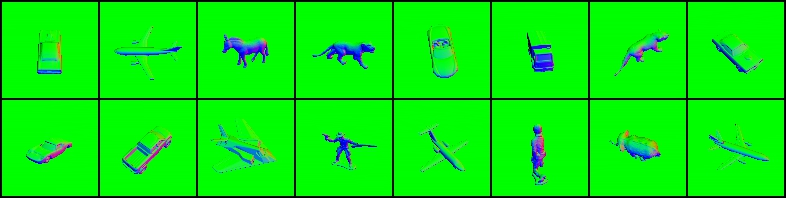
\includegraphics[width=1.0\textwidth]{./assets/synth_world_normals.jpg}
\caption{World Space Normals Map in RGB}
\label{fig:GBUFFER_NORMALS}
\end{figure}

\item Albedo

\begin{figure}[h!]
\centering
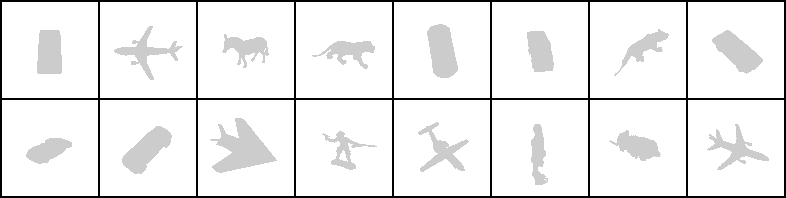
\includegraphics[width=1.0\textwidth]{./assets/synth_albedo.jpg}
\caption{Albedo Map}
\label{fig:GBUFFER_ALBEDO}
\end{figure}

\item Positions

\begin{figure}[h!]
\centering
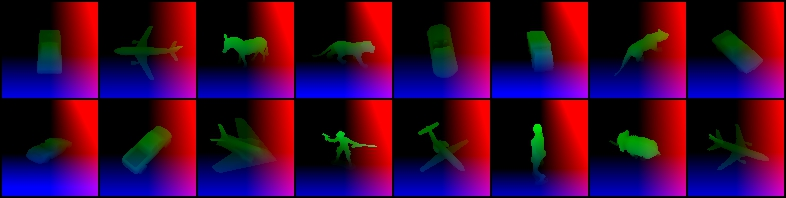
\includegraphics[width=1.0\textwidth]{./assets/synth_world_positions.jpg}
\caption{Albedo Map}
\label{fig:GBUFFER_POSITIONS}
\end{figure}

\item Depth

\begin{figure}[h!]
\centering
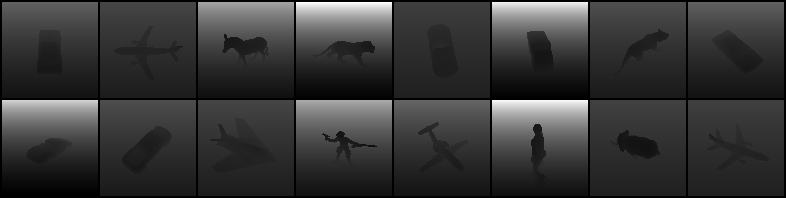
\includegraphics[width=1.0\textwidth]{./assets/synth_linear_depth.jpg}
\caption{Depth Map}
\label{fig:GBUFFER_DEPTH}
\end{figure}

\item Shadow (only one)

\begin{figure}[h!]
\centering
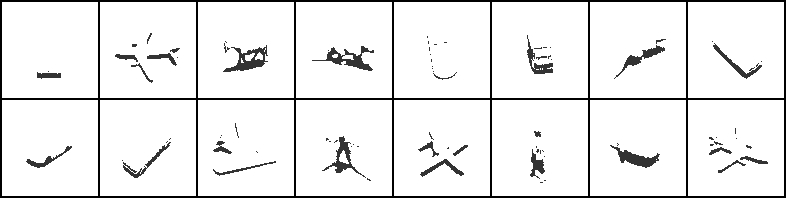
\includegraphics[width=0.8\textwidth]{./assets/synth_occlusion1.jpg}
\caption{Shadow Map}
\label{fig:GBUFFER_SHADOW}
\end{figure}

\begin{figure}[h!]
\centering
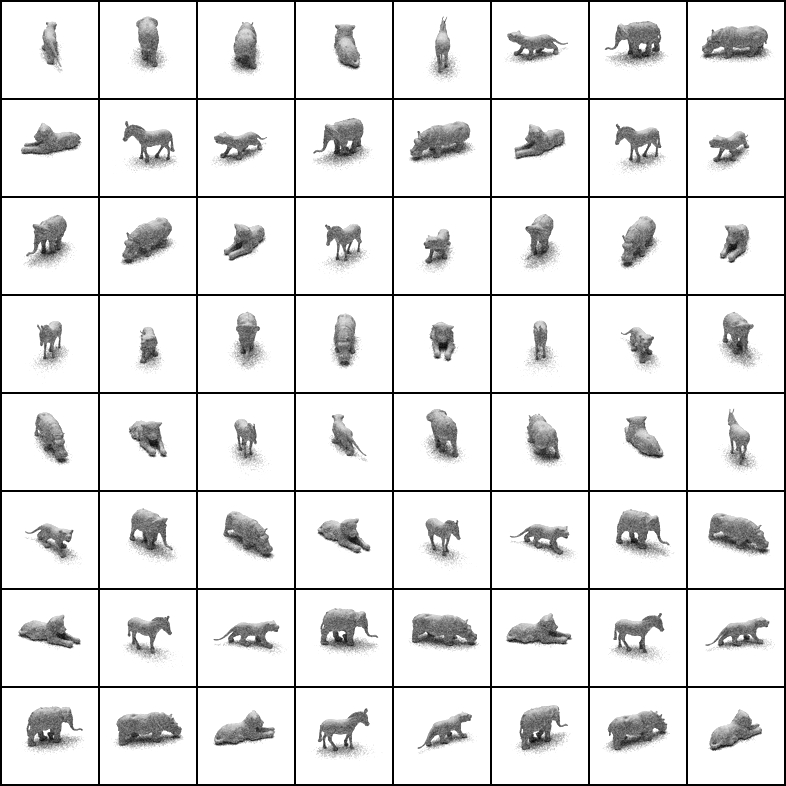
\includegraphics[trim={0 0 392px 687px},clip,width=1.0\textwidth]{./assets/traindata_1_sample.jpg}
\caption{Sample crop 1.}
\label{fig:crop1}
\end{figure}
\begin{figure}[h!]
\centering
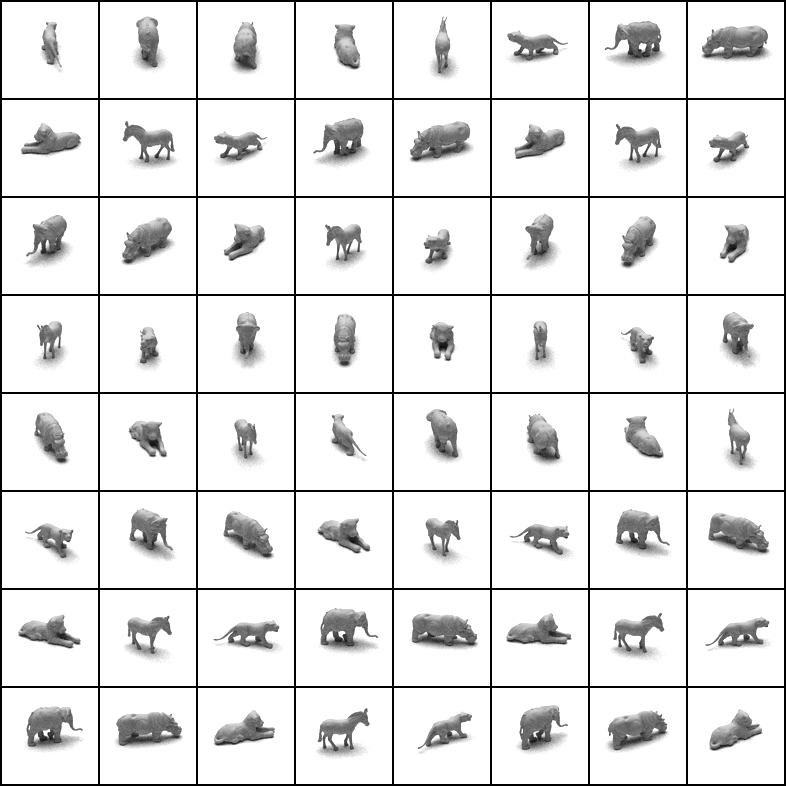
\includegraphics[trim={0 0 392px 687px},clip,width=1.0\textwidth]{./assets/traindata_4_sample.jpg}
\caption{Sample crop 4.}
\label{fig:crop4}
\end{figure}
\begin{figure}[h!]
\centering
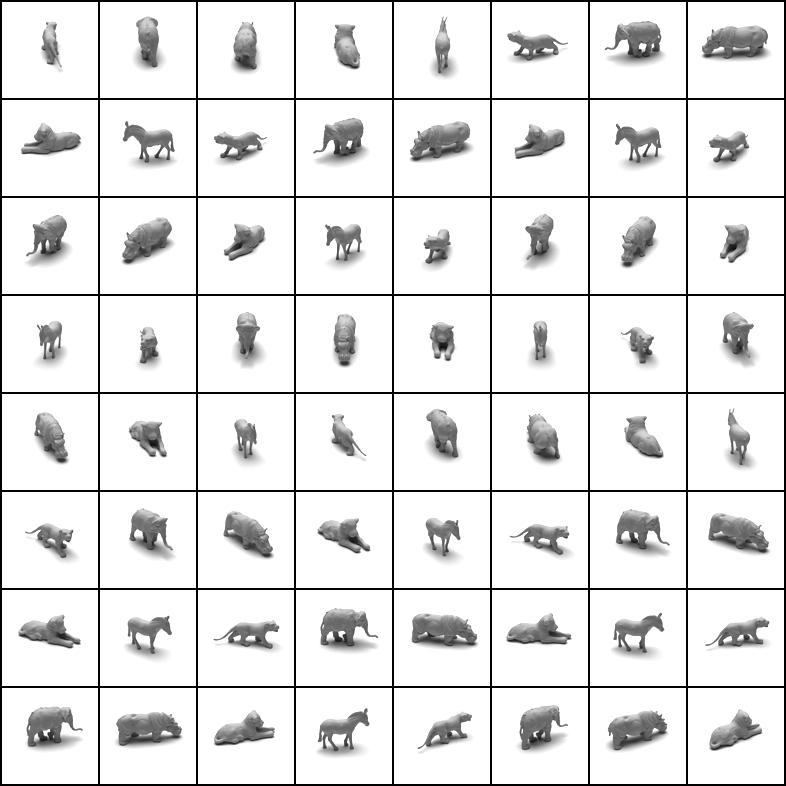
\includegraphics[trim={0 0 392px 687px},clip,width=1.0\textwidth]{./assets/traindata_target_128_sample.jpg}
\caption{Sample crop 128.}
\label{fig:crop128}
\end{figure}

\end{itemize}
\end{comment}

\bibliography{bibliography}{}
\bibliographystyle{plain}
\end{document}
